% ============================================
% Thesis Template – Uniba Collab Thesis Template
% Developed and maintained by Giulio Mallardi
% https://collab.uniba.it | © 2025 Collab
% ============================================
\PassOptionsToPackage{table, dvipsnames}{xcolor}
\documentclass[a4paper,twoside,12pt]{toptesi}

% ensure encoding and babel come before soul
\usepackage[T1]{fontenc}
\usepackage[utf8]{inputenc}
\usepackage[italian]{babel}

% load soul after encoding; register fragile commands used inside \hl
\usepackage{soul}   % provides \hl
\usepackage{xcolor} % color configuration

\soulregister\cite7
\soulregister\ref7
\soulregister\label7
\soulregister\textbf7
\soulregister\emph7

\usepackage{graphicx}
\usepackage{tikz}
\usetikzlibrary{positioning}
\usepackage{pgfplots}
\usepackage[newfloat]{minted}
\usepackage[font=small,skip=1pt]{caption}
\usepackage{subcaption}
\pgfplotsset{compat=1.18}
\usepackage{hyperref}
\usepackage{booktabs}
\hypersetup{
    colorlinks = true,
    allcolors=black
}
\usepackage{amsfonts}

% prevent \hl from breaking PDF bookmarks
\pdfstringdefDisableCommands{\renewcommand{\hl}[1]{#1}}
%This equals 1.5 linespacing in Word
\linespread{1.25}
% Include and number subsubsections in the ToC
\setcounter{secnumdepth}{3}
\setcounter{tocdepth}{3}

\usepackage{fancyhdr} % nel preambolo, se non già incluso
\usepackage{graphicx} % per il logo
\usepackage{ifthen}   % per i controlli condizionali (facoltativo ma utile)
\usepackage{amsmath}
\usepackage{algorithm}
\usepackage{algpseudocode}
\usepackage{longtable}
\usepackage{booktabs}
\usepackage{rotating}  % Per l'ambiente sidewaystable
\usepackage{booktabs}  % Per linee di tabella professionali (\toprule, \midrule, \bottomrule)
\usepackage{tabularx}  % Per colonne di tipo 'X' che si adattano alla larghezza
\def\dept{DIPARTIMENTO DI INFORMATICA}
\def\course{CORSO DI LAUREA IN INFORMATICA}
%\def\course{CORSO DI LAUREA IN INFORMATICA E \\ TECNOLOGIE PER LA PRODUZIONE DEL SOFTWARE}
%\def\course{CORSO DI LAUREA MAGISTRALE IN INFORMATICA}
%\def\course{CORSO DI LAUREA MAGISTRALE IN SICUREZZA INFORMATICA}
\def\title{Valutazione degli effetti di adversarial poisoning  sull’addestramento di un modello per la scoperta di Windows PE malware}
\def\author{Mauro Losurdo}
\def\relatoreone{Prof.ssa Andresini Giuseppina}

\def\subject{INTELLIGENZA ARTIFICIALE NELLA SICUREZZA INFORMATICA }
\def\annoacc{2024 - 2025}
\def\beforecandidate{LAUREANDO:}
\def\beforetitle{TESI DI LAUREA \\ IN \\ }
\def\beforeprof{RELATORE:}
\def\beforecorrelatore{CORRELATORI:}
\def\beforeannoacc{ANNO ACCADEMICO}
\usepackage{xspace}

\makeatletter
\def\cleardoublepage{\clearpage\if@twoside \ifodd\c@page\else
    \hbox{}
    \vspace*{\fill}
    \vspace{\fill}
    \thispagestyle{empty}
    \newpage
    \if@twocolumn\hbox{}\newpage\fi\fi\fi}
\makeatother


\begin{document}

\begin{titlepage}
	\begin{tikzpicture}[remember picture,overlay]
		\centering
		\node[yshift=-6 cm] (logo) at (current page.north) {\includegraphics[width=0.75\linewidth]{images/uniba.jpg}};
			\node[text width=50em,yshift=0.25cm, align = center, below = of logo](dipartimento){\normalsize \dept};
			\node[text width=40em, align = center, yshift=.55cm,below = of dipartimento](course){\normalsize \course};
		\node[text width=35em,align = center,  yshift=1.2cm,below = of course](line){\par\noindent\rule{\textwidth}{0.4pt}};
		\node[text width=40em, align = center, yshift=.55cm,below = of line](lia){\normalsize \beforetitle \xspace \subject };
		
  \node[text width=40em, align = center, yshift=-0.5cm,below = of lia](title){\bfseries \parbox{12cm}{\fontsize{21pt}{20pt}\selectfont \centering \title\par}};
  
	\node[text width=35em, align = left, yshift=-1cm,below = of title](relatoretit){\normalsize \textbf{\beforeprof} };
 	\node[text width=35em, align = left, yshift=1cm,below = of relatoretit](relatore){\large \relatoreone };


      
		\node[text width=35em, align = right, yshift=-1cm,below = of title](candidatetit){\normalsize \textbf{\beforecandidate}};
		 \node[text width=35em, align = right, yshift=1cm,below = of candidatetit](candidate){\large \author};

  \node[text width=35em,align = center,  yshift= -3cm,below = of candidate](line2){\par\noindent\rule{\textwidth}{0.4pt}};
	
  
  \node[text width=50em, align = center, yshift=0.5cm,below = of line2](year){\large \beforeannoacc\xspace \annoacc};
	\end{tikzpicture}
\end{titlepage}


\cleardoublepage

% \begin{dedication}
    \begin{flushright}
        {\small % Cambia la dimensione del font qui
            \textit{``Lorem ipsum dolor sit amet, consectetur adipiscing elit...\\
            Sed nemo scit quid significet, quia Ciceronem mutilatum est.'' \\ 
            --- Marcus Tullius Cicero \\[2em]
            \footnotesize Dedico questo lavoro a chi fingerà di capire questi placeholder latini}
        }
    \end{flushright}
\end{dedication}

\cleardoublepage
\pagenumbering{roman}

\tableofcontents

\cleardoublepage

\pagenumbering{arabic}
\setcounter{page}{1}
\chapter*{Disclaimer}
Tutti i marchi, nomi commerciali, prodotti e loghi menzionati in questo elaborato sono di proprietà dei rispettivi titolari. 
L’autore non rivendica alcun diritto su tali marchi o nomi commerciali e li utilizza esclusivamente a scopo informativo e descrittivo, senza alcun intento di violazione.

% % --- Definizione del footer personalizzato per il Disclaimer ---
% \fancypagestyle{collabfooter}{
%   \fancyhf{} % pulisce header e footer
%   \fancyfoot[C]{%
%       \vspace{-3cm} % alza il footer di circa 1 cm

%     \IfFileExists{images/collab.png}{%
%       \includegraphics[width=2.2cm]{images/collab.png}\\[12pt]
%     }{}%
%     {\scriptsize
%       Questa tesi è stata realizzata nell’ambito delle attività di ricerca del\\ 
%         \textbf{}\\
%       \textbf{Collab – Collaborative Development Group}\\
%       Dipartimento di Informatica, Università degli Studi di Bari Aldo Moro
%     }%
%   }
%   \renewcommand{\headrulewidth}{0pt}
%   \renewcommand{\footrulewidth}{0pt} % linea sottile sopra il footer (facoltativa)
% }

% \thispagestyle{collabfooter}
% Configurazione dello stile
\vfill % Spinge tutto quello che segue in fondo alla pagina

\begin{center}
        %  \includegraphics[width=2.2cm]{images/kddeHDLogo.png}\\[5pt]
    {}%
    {\scriptsize
        Questa tesi è stata realizzata nell’ambito delle attività di ricerca del\\ 
        \textbf{KDDE - Knowledge Discovery and Data Engineering}\\
        Dipartimento di Informatica, Università degli Studi di Bari Aldo Moro
    }
\end{center}'


\cleardoublepage
\addcontentsline{toc}{chapter}{Introduzione}
\chapter*{Sommario}

L'Intelligenza Artificiale, pur essenziale per la malware detection, rimane vulnerabile agli attacchi adversarial. Questa tesi indaga la robustezza dei classificatori per file Windows PE contro il \textit{Data Poisoning}, focalizzandosi sul obiettivo di indurre falsi positivi trasformando file legittimi in minacce apparenti, minando così la fiducia nel sistema di rilevamento.

Attraverso il confronto degli algoritmi black-box \textit{GAMMA} e \textit{OLIVANDER}, sono state testate strategie di \textit{Label Flipping} e \textit{Clean Label} per avvelenare un modello bersaglio. I risultati evidenziano che solo il Label Flipping compromette efficacemente le prestazioni, mentre il Clean Label agisce involontariamente come rafforzamento del modello. Lo studio conferma inoltre l'elevata efficacia di OLIVANDER, la trasferibilità degli attacchi tra diverse architetture e la loro capacità di eludere anche validazioni esterne come VirusTotal.

\chapter{Introduzione}
\label{cap:introduzione}

La sicurezza informatica mira a proteggere sistemi e dati da attività ostili. Con
il termine “malware” si indicano file o porzioni di codice progettati per compromettere
i sistemi ottenendo accessi non autorizzati, esfiltrando informazioni, interrompendo
servizi o danneggiando reti. Negli ultimi anni, l’Intelligenza Artificiale (IA) ha
assunto un ruolo centrale nel rilevamento del malware: modelli di Machine
Learning (ML) e Deep Learning (DL) hanno consentito di raggiungere livelli di
accuratezza elevati, migliorando la capacità dei sistemi anti‑malware di riconoscere
minacce anche mai osservate prima.

Parallelamente, anche gli avversari hanno evoluto le proprie tecniche. Nel 2024,
ad esempio, i sistemi di rilevamento di Kaspersky hanno registrato in media 467,000
nuovi campioni malevoli al giorno, con un incremento significativo del 14\% rispetto al
2023. Nello stesso periodo, Microsoft Windows è rimasto l’obiettivo privilegiato,
rappresentando il 93\% dei dati infetti rilevati quotidianamente\cite{kaspersky2024maliciousfiles}. In questo contesto,
la presente tesi si concentra sui malware in formato Portable Executable (PE)
per la piattaforma Windows.

Nonostante i recenti progressi, i modelli decisionali basati su IA presentano vulnerabilità
strutturali agli attacchi Adversarial: piccole perturbazioni intenzionali
applicate all'input possono indurre il modello a produrre classificazioni errate,
consentendo l'evasione dei meccanismi di difesa. Questo lavoro esplora tali
vulnerabilità nel dominio dei file Windows PE. 

In particolare, questa tesi confronta due algoritmi di poisoning, \textit{Olivander} 
e \textit{Gamma}, in uno scenario atipico rispetto alla letteratura tradizionale. 
Invece di perturbare campioni della classe \textit{Malware} per farli classificare 
erroneamente come \textit{Goodware} (il caso tipico di evasione), invertiamo la 
prospettiva: modifichiamo file legittimi (\textit{Goodware}) con l'obiettivo di 
indurre il classificatore a etichettarli come \textit{Malware}. Questo approccio 
permette di studiare la robustezza dei modelli di rilevamento rispetto a falsi 
positivi sistematici e analizzare come tecniche di poisoning possano compromettere 
la fiducia nei sistemi anti-malware.

% \section{Contributi}

% I principali contributi di questa tesi sono i seguenti:

% \begin{itemize}
%     \item \textbf{Analisi comparativa di algoritmi di poisoning}: confrontiamo le prestazioni 
%     di \textit{Olivander} e \textit{Gamma} in uno scenario invertito, valutando la loro capacità 
%     di trasformare file Goodware in campioni classificati come Malware, misurando l'efficacia 
%     delle perturbazioni generate e il loro impatto sulla funzionalità dei file.
    
%     \item \textbf{Studio della robustezza dei modelli}: analizziamo la vulnerabilità dei 
%     classificatori basati su Machine Learning agli attacchi di poisoning, con particolare 
%     attenzione alla generazione di falsi positivi sistematici che possono minare la fiducia 
%     degli utenti nei sistemi di sicurezza.
    
%     \item \textbf{Valutazione della trasferibilità degli attacchi}: studiamo se i campioni 
%     perturbati generati contro un modello specifico mantengono la loro efficacia quando 
%     testati su classificatori diversi o su sistemi anti-malware commerciali, fornendo 
%     indicazioni sulla generalizzabilità degli attacchi di poisoning.
    
%     \item \textbf{Analisi delle caratteristiche sfruttate}: esaminiamo quali feature dei 
%     file Windows PE vengono maggiormente manipolate dagli algoritmi di poisoning per 
%     ottenere la riclassificazione desiderata, offrendo insight utili per lo sviluppo 
%     di contromisure più robuste.
% \end{itemize}

\section{Contributi}

Il resto di questa tesi è organizzato come segue:

\begin{itemize}
    \item \textbf{Capitolo 2 - Background}: introduce i concetti fondamentali necessari 
    alla comprensione del lavoro, inclusi il formato Windows PE, l'utilizzo della libreria 
    LIEF per l'analisi statica dei file eseguibili, e una descrizione degli algoritmi 
    di attacco black-box che preservano la funzionalità, con particolare focus su 
    \textit{GAMMA} e \textit{Olivander}.
    
    \item \textbf{Capitolo 3 - Stato dell'arte}: presenta una panoramica della letteratura 
    recente sull'adversarial learning e sulle tecniche di poisoning applicate ai sistemi 
    di rilevamento malware, posizionando il presente lavoro nel contesto della ricerca 
    attuale.
    
    \item \textbf{Capitolo 4 - Poisoning in Machine Learning}: approfondisce l'utilizzo 
    di tecniche di Machine Learning e Deep Learning per la malware detection, descrivendo 
    come vengono estratte le feature dai file PE tramite LIEF e illustrando le metodologie 
    di poisoning applicate, incluse le strategie di manipolazione delle label e le tecniche 
    di perturbazione utilizzate negli esperimenti.
    
    \item \textbf{Capitolo 5 - Valutazione sperimentale}: descrive il dataset utilizzato, 
    i dettagli implementativi dei modelli di classificazione e degli algoritmi di attacco, 
    e presenta un'analisi dettagliata dei risultati ottenuti, includendo valutazioni di 
    baseline e studi sulla trasferibilità degli attacchi verso classificatori diversi.
    
    % \item \textbf{Capitolo 6 - Conclusioni}: riassume i risultati principali della ricerca, 
    % discute le implicazioni per la sicurezza dei sistemi di rilevamento malware basati su 
    % IA, e delinea possibili direzioni per lavori futuri.
\end{itemize}

\chapter{Background}
In questo capitolo vengono descritte le basi teoriche necessarie per introdurre il lavo
ro svolto. In particolare i concetti su cui si basano GAMMA e Olivander, i due algoritmi usati in questo caso di studio.

\section{File Windows PE}
Il formato Portable Executable (PE) costituisce lo standard de facto per i file eseguibili, il codice oggetto,
le librerie a collegamento dinamico (DLL) e altri file immagine utilizzati nelle versioni a 32 e 64 bit dei sistemi 
operativi Microsoft Windows.\cite{PeFormatDocs}


Lo standard è condiviso sia per i file eseguibili (detti `image`) e gli object-file;per lo scopo della tesi sono di interesse solo i file eseguibili

\subsection{Struttura generale}
Un file PE è organizzato in una struttura gerarchica composta da header, tabelle di dati e sezioni. 
La struttura può essere suddivisa nei seguenti componenti principali\cite{PeFormatDocs}:

\begin{itemize}
    \item \textbf{DOS Header e DOS Stub}: per compatibilità con sistemi MS-DOS legacy, viene inserito un eseguibile segnaposto (stub) per i sistemi DOS, che stampa a schermo la stringa \texttt{This program cannot be run in DOS mode}, e un puntatore all'header PE
    \item \textbf{PE HEADER}: firma (signature) del file PE (\texttt{PE\textbackslash0\textbackslash0}, le lettere ``P'' ed ``E'' seguite da due null-byte) e la intestazione del file (IMAGE\_FILE\_HEADER) che contiene informazioni sulla compilazione
    \item \textbf{COFF File Header}: informazioni sulla architettura target, numero di sezioni e caratteristiche generali
    \item \textbf{Optional Header}: metadati essenziali per il caricamento, per esempio se l'architettura target è a 32 o 64bit, versione, Checksum etc..
    \item \textbf{Section Table}: array di descrittori delle sezioni
    \item \textbf{Sections}: il contenuto effettivo del programma organizzato in sezioni
\end{itemize}

\begin{figure}[ht]
    \centering
    \includegraphics[width=0.8\textwidth]{images/pe-structure.png}
    \caption{Struttura generale di un file PE: dal header DOS alle sezioni\cite{MZRSTpeStructure}}
    \label{fig:pe-structure}
\end{figure}

\subsubsection{Le sezioni in un file PE}
Contenute dopo tutti gli header di un file PE,le sezioni rappresentano i blocchi funzionali in cui è suddiviso il contenuto di un file PE, e ne occupano il resto del contenuto.Ogni sezione 
è descritta da una entry nella Section Table (struttura \texttt{IMAGE\_SECTION\_HEADER}) che specifica le sue proprietà principali, riassunte nella tabella seguente:

\begin{table}[H]
\caption{Descrittore di una sezione}
\label{tab:section-header}
\centering
\begin{tabular}{@{}p{0.25\textwidth}p{0.70\textwidth}@{}}
\toprule
\textbf{Campo} & \textbf{Descrizione} \\
\midrule
\textbf{Name} & Nome della sezione (fino a 8 caratteri). \\
\textbf{VirtualSize} & Dimensione della sezione quando caricata in memoria. \\
\textbf{VirtualAddress} & Indirizzo relativo della sezione in memoria (RVA). \\
\textbf{SizeOfRawData} & Dimensione della sezione su disco (allineata a \texttt{FileAlignment}). \\
\textbf{PointerToRawData} & Offset fisico della sezione nel file. \\
\textbf{Characteristics} & Flag che definiscono gli attributi: leggibile, scrivibile, eseguibile, contenuto codice/dati, condivisibile, eliminabile dalla memoria, ecc. \\
\bottomrule
\end{tabular}
\end{table}

Le sezioni consistono di semplici blocchi di byte. Le sezioni standard più comuni sono riassunte nella seguente tabella:

\begin{table}[H]
\caption{Sezioni standard più comuni in un file PE}
\label{tab:pe-sections}
\centering
\begin{tabular}{@{}p{0.15\textwidth}p{0.78\textwidth}@{}}
\toprule
\textbf{Nome} & \textbf{Descrizione} \\
\midrule
\texttt{.text} & Contiene il codice eseguibile del programma. Questa sezione è tipicamente marcata come eseguibile e di sola lettura. È la sezione principale dove risiede la logica dell'applicazione. \\
\texttt{.data} & Contiene dati inizializzati e scrivibili. Include variabili globali e statiche con valori iniziali definiti nel codice sorgente. \\
\texttt{.rdata} & Contiene dati di sola lettura, come costanti stringa, tabelle di virtual function (vtable) e la Import Address Table (IAT). \\
\texttt{.bss} & Contiene dati non inizializzati. Occupa spazio in memoria ma non nel file su disco, poiché verrà azzerata al caricamento. \\
\texttt{.rsrc} & Contiene le risorse del programma: icone, bitmap, stringhe localizzate, menu, dialog box e altri elementi dell'interfaccia utente. \\
\texttt{.reloc} & Contiene informazioni di rilocazione necessarie per l'Address Space Layout Randomization (ASLR). Permette al loader di modificare gli indirizzi quando il programma non può essere caricato al suo indirizzo base preferito. \\
\texttt{.edata} & Contiene la Export Directory Table per DLL che esportano funzioni utilizzabili da altri moduli. \\
\texttt{.idata} & Contiene la Import Directory Table con informazioni sulle funzioni importate da altre DLL. \\
\texttt{.pdata} & Contiene informazioni per la gestione delle eccezioni. \\
\texttt{.tls} & Contiene dati per variabili thread-specific. (Thread Local Storage) \\
\bottomrule
\end{tabular}
\end{table}

\paragraph{Sezioni personalizzate}
Oltre alle sezioni standard, un file PE può contenere sezioni personalizzate con nomi arbitrari. 
Il formato è estremamente flessibile: le sezioni non devono seguire un ordine particolare, 
possono avere dimensioni diverse su disco e in memoria, e possono contenere spazi non utilizzati.

\begin{figure}[ht]
    \centering
    \includegraphics[width=0.8\textwidth]{images/winInternal.png}
    \caption{Sezioni di un file PE, viste da winInternal}
    \label{fig:winInternal}
\end{figure}

% Questa flessibilità rende le sezioni PE un obiettivo privilegiato per tecniche di evasione e 
% offuscamento. Gli attaccanti possono:

% \begin{itemize}
%     \item Aggiungere sezioni personalizzate con payload malevoli
%     \item Modificare i permessi delle sezioni esistenti
%     \item Nascondere dati negli spazi non utilizzati tra le sezioni
%     \item Manipolare i descrittori mantenendo la funzionalità del file
%     \item Sfruttare discrepanze tra VirtualSize e SizeOfRawData
%     \item Alterare l'entry point per eseguire codice da sezioni non standard
% \end{itemize}

% Queste caratteristiche rendono il formato PE particolarmente interessante per gli attacchi 
% adversarial che mirano a evadere i sistemi di rilevamento basati su machine learning, 
% come verrà approfondito nei capitoli successivi.

\section{LIEF per l'analisi statica dei file windows PE}
\label{LIEF_data}
LIEF (Library to Instrument Executable Formats) è una libreria open-source ampiamente utilizzata 
per la manipolazione e l'analisi statica di file binari, con particolare supporto per il formato 
Windows PE\cite{LIEF}. Sviluppata originariamente da Quarkslab, LIEF fornisce un'interfaccia 
unificata per lavorare con diversi formati eseguibili (PE, ELF, Mach-O). 

LIEF è stato usato per estrarre 2381 caratteristiche~(feature) del dataset EMBER~\cite{2018arXiv180404637A}
Dal suo rilascio, il dataset originale EMBER  è stato citato più di 600 volte,da più di  350  istituzioni citanti uniche  in 6 continenti~\cite{Joyce_2025}.\linebreak
Le caratteristiche analizzate si possono dividere in 9 gruppi: \label{feature_set}

\subsection{Informazioni dal formato PE}
\paragraph{Informazioni generali sul file} (10 feature) in questo gruppo sono incluse le caratteristiche recuperabili dal intestazione del file PE, quindi la grandezza del eseguibile una volta mappato su memoria virtuale, il numero di funzioni importate ed esportate, presenza di determinate sezioni,risorse, etc ..
\paragraph{Informazioni dal COFF/Optional Header} (62 feature) in questo gruppo sono incluse le caratteristiche recuperabili dall'header COFF e dall'header opzionale, dato che le informazioni contenute in questi header sono principalmente in formato stringa o lista di stringhe vengono sintetizzati utilizzando la tecnica del feature hashing\cite{hashTrick} (chiamato anche hash-trick) con 10 bin allocati per ciascun noise-vector.
\paragraph{Informazioni sulle funzioni importate} (1280 feature) in questo gruppo sono incluse le caratteristiche recuperabili analizzando la IAT raggruppate per libreria di origine. anche qui le stringhe \texttt{funzione:libreria} sono compresse usando l'hashTrick (256 bins per le librerie, 1024 per le funzioni).
\paragraph{Informazioni sulle funzioni esportate} (128 feature) in questo gruppo sono incluse le caratteristiche recuperabili analizzando la EAT, riassunte tramite hashTrick in 128 bins
\paragraph{Informazioni sulle sezioni} (255 feature) descrive i dati registrati nell'header delle sezioni (es. nome, dimensione, entropia, VirtualSize), con particolare attenzione alla sezione che contiene l'entry point.
\paragraph{Informazioni sulla Data Directory} (30 feature) descrive i valori di Size e VirtualSize di tutte le voci della Data Directory registrate nel file PE.
\subsection{Informazioni agnostiche del formato}
\paragraph{Istogramma dei byte} (256 feature)
L'istogramma dei byte contiene 256 valori interi che rappresentano il conteggio di ciascun 
valore di byte presente nel file, questo istogramma viene normalizzato a una distribuzione rispetto la dimensione del file, cioè
\[
h_i = \frac{c_i}{N}, \qquad i = 0,\dots,255
\]
dove \(c_i\) è il conteggio del byte di valore \(i\) e \(N\) è il numero totale di byte nel file.

Esempio: consideriamo un file con in cui il  byte (in esadecimale) 0x42 si ripete 500 volte, e il file è lungo 2000 byte, la distribuzione normalizzata per \(h_{0x42}\) è 0.25.
\paragraph{Istogramma dei byte-entropia} (256 feature)
L'istogramma byte-entropia approssima la distribuzione congiunta \(p(H, X)\) dell'entropia \(H\) e 
del valore byte \(X\) come descritto in~\cite{saxe2015deepneuralnetworkbased}. 
calcolando l'entropia scalare \(H\) per una finestra a lunghezza fissa e associandola a ogni occorrenza di byte all'interno della finestra. L'operazione viene ripetuta facendo scorrere la finestra sui byte di input. Nella nostra implementazione utilizziamo una finestra di 2048 byte e uno step di 1024 byte, con \(16 \times 16\) bin che quantizzano l'entropia e il valore del byte. Prima dell'addestramento normalizziamo questi conteggi in modo che la loro somma sia pari a uno.
%30 e 255
\paragraph{Informazioni sulle stringhe} (104 feature)

Il dataset include statistiche semplici sulle stringhe stampabili che sono lunghe almeno cinque caratteri stampabili. In particolare, vengono 
riportati il numero di stringhe, la loro lunghezza media, un istogramma dei caratteri stampabili presenti 
in tali stringhe e l'entropia dei caratteri su tutte le stringhe stampabili. Inoltre, il gruppo  include il numero di stringhe che iniziano con \texttt{C:\textbackslash} (senza 
distinzione tra maiuscole e minuscole) che possono indicare un percorso, il numero di occorrenze di 
\texttt{http://} o \texttt{https://} (senza distinzione tra maiuscole e minuscole) che possono indicare 
un URL, il numero di occorrenze di \texttt{HKEY\_} che possono indicare una chiave di registro, e il 
numero di occorrenze della stringa \texttt{MZ} che può fornire una debole evidenza di un dropper 
di eseguibili Windows PE o di eseguibili in bundle.

\section{Attacchi Black-box che preservano la funzionalità}
% aggiunere tutta la teoria qui


\subsection{Problema dell'apprendimento predittivo nel caso di un problema di classificazione}

Il machine learning (ML) è un campo dell'informatica che mira a insegnare ai computer come apprendere e agire senza essere esplicitamente programmati.\cite{deepAImlGlossary}

Un sistema di machine learning addestrato per un problema di classificazione tenta di trovare una funzione ipotesi
\(f\) che mappa gli eventi nelle diverse classi.\cite{10.1145/1128817.1128824}

Un problema di apprendimento predittivo (supervisionato) è definito su uno spazio di input \(X\), uno spazio di output $Y$
e una funzione di perdita \(\ell : Y \times Y \to \mathbb{R} \).
L'input al problema è un insieme di addestramento \(S\), specificato come
\( \{(x_i, y_i) \in X \times Y\} \), e l'output è una funzione ipotesi \(f : X \to Y\).
Scegliamo \(f\) da uno spazio di ipotesi (o classe di funzioni) \(\mathcal{F}\) per minimizzare
l'errore di predizione definito dalla funzione di perdita.
Durante l'addestramento di un modello di machine learning l'obiettivo è minimizzare la funzione di perdita su un insieme di dati di addestramento come riportato nell'Equazione \ref{eq:learning}. La stazionarietà permette di ridurre il
problema di apprendimento predittivo alla minimizzazione della somma delle perdite sull'insieme
di addestramento\cite{10.1145/1128817.1128824}:

\begin{equation}
f^{\ast} = \arg\min_{f \in \mathcal{F}} \sum_{(x_i,y_i)\in S} \ell\big(f(x_i), y_i\big)
\label{eq:learning}
\end{equation}


\subsection{Adversarial attacks}

L'adozione rapidamente in espansione delle tecnologie ML, tuttavia,
 ha reso questi sistemi obiettivi attraenti per gli avversari che desiderano
 manipolare tali meccanismi per scopi malevoli\cite{liu2017neural}.
L'addestramento di un sistema di ML si fonda sull'utilizzo di dataset che si presumono rappresentativi e affidabili per il dominio di interesse. Questa condizione è necessaria affinché il modello possa fornire risultati validi. Tuttavia, gli attori malintenzionati possono influenzare gli algoritmi decisionali di tali approcci andando a modificare i dati di addestramento oppure forzando il modello a produrre l'output desiderato, ad esempio la classificazione errata di eventi anomali,consentendo agli avversari di ridurre significativamente le prestazioni complessive, causare classificazioni errate mirate o comportamenti indesiderati\cite{PITROPAKIS2019100199}


\subsubsection{Adversarial machine learning}
\label{cap2:adm}
L'Adversarial machine learning (AML) è un campo di ricerca nell'ambito dell'intelligenza artificiale, si trova all'intersezione tra l'apprendimento automatico e la sicurezza informatica, ed è spesso definito
come lo studio di tecniche di attacco apprendimento automatico efficaci contro
un avversario.\cite{huang2016learningstrongadversary}

Sebbene la letteratura evidenzi la 'dualità' di questo campo\cite{saini2024reviewdualityadversariallearning}, che comprende anche lo sviluppo di contromisure difensive, questo lavoro si focalizzerà sulla componente offensiva. In questo contesto, l'avversario cerca di sfruttare le vulnerabilità dei modelli di machine learning per raggiungere i propri scopi.
L'interazione tra avversario e il modello è modellabile come un gioco non-cooperativo (specificamente un Duopolio di Stackelberg\cite{5360532}) dove il modello ha come obiettivo il minimizzare la sua \textit{loss function}, mentre l'obbiettivo dell'avversario è quello di massimizzare l'impatto del attacco cioè massimizzare la  \textit{loss function} del modello, tenendo conto di una funzione di costo basata sulla distanza tra un evento valido e un evento creato dall'avversario.\cite{PITROPAKIS2019100199}

Operativamente, un attacco adversarial  si concretizza nella generazione di \textit{adversarial examples}: istanze di dati appositamente modificate per ingannare il classificatore, massimizzando l'errore di predizione senza alterare il contenuto semantico percepibile dall'osservatore.

\subsubsection{Tassonomia attacchi adversarial}

Mentre i dettagli di implementazioni di attacchi contro ML possono variare di molto, possono essere classificati secondo una tassonomia descritta in figura~\ref{fig:taxonomy}, in seguito dettagliata:
\begin{figure}[t!]
    \centering
    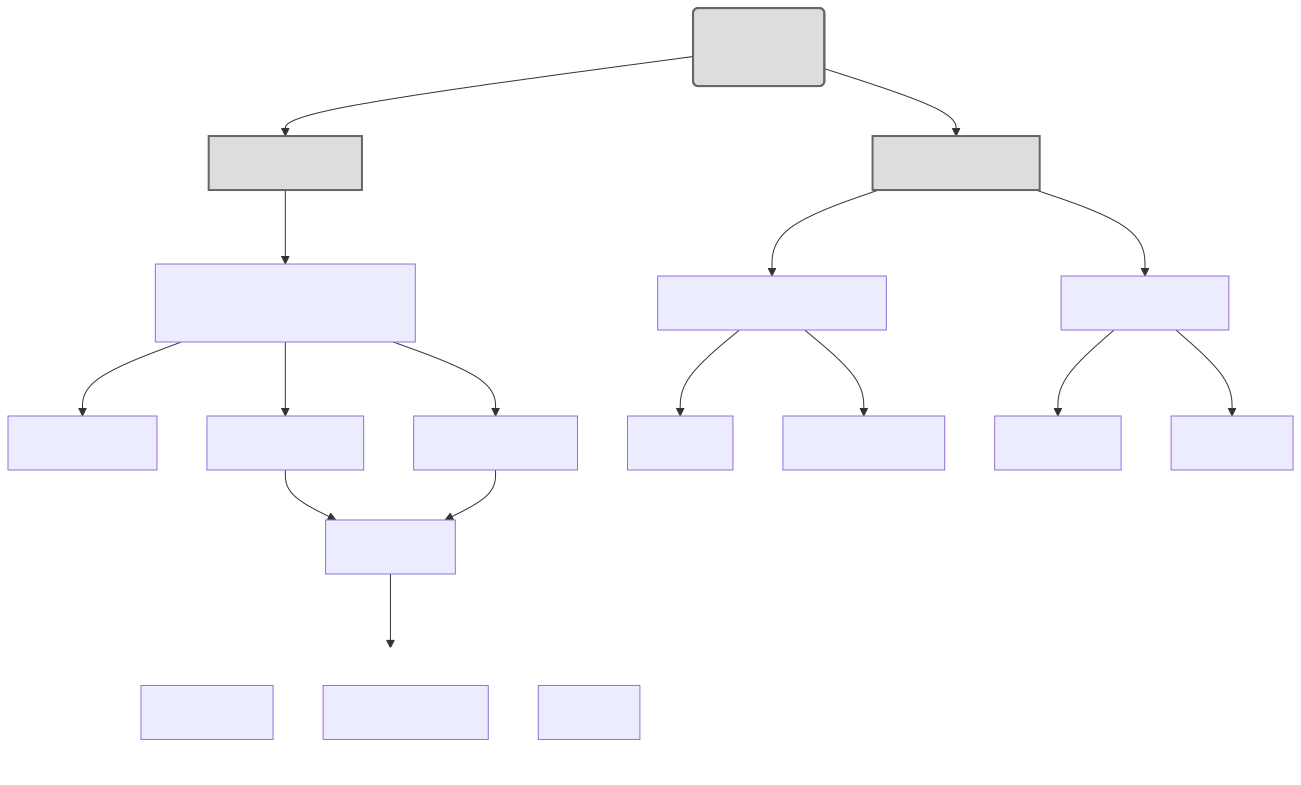
\includegraphics[width=0.9\textwidth]{images/taxonomy-1.png}
    \caption{tassonomia dei attacchi verso modelli di machine learning}
    \label{fig:taxonomy}
\end{figure}


\paragraph{Conoscenza dell'attacante} in base alla conoscenza che l'attaccante possiede del modello di machine learning, gli attacchi possono essere classificati in tre categorie principali:

\begin{itemize}
    \item \textbf{White-box attacks}: L'attaccante ha accesso completo alla struttura del modello, ai parametri, ai pesi, alle funzioni di attivazione e all'algoritmo di training. Questa è la situazione più favorevole per l'attaccante, in quanto può calcolare esattamente come il modello risponde agli input e progettare attacchi altamente efficaci basati su questa conoscenza completa.
    
    \item \textbf{Black-box attacks}: L'attaccante non ha accesso diretto al modello, ma può solo interrogarlo fornendo input e osservando gli output predetti. In questo scenario, l'attaccante deve inferire il comportamento del modello attraverso query ripetute
    
    \item \textbf{Grey-box attacks}: L'attaccante possiede conoscenza parziale del modello. Questo potrebbe includere l'architettura generale del modello, alcuni parametri, informazioni sulla fase di training, oppure accesso a un modello surrogato simile. Questa situazione rappresenta uno scenario intermedio tra gli attacchi white-box e black-box.
\end{itemize}


\paragraph{Specificità dell'attacco}

Se l'obiettivo dell'attaccante è quello che l'esempio generato sia misclassificato in una specifica classe si parla di attacco mirato (\textit{Error-specific attack}) se invece in una classe diversa dall'originale si parla di attacco indiscriminato (\textit{Error-generic})\cite{10.1145/1128817.1128824}

\paragraph{Tempo di attacco}
Un attacco è classificato in base a che fase (training o test) ha come obbiettivo:\cite{10.1145/1128817.1128824}

\begin{itemize}
    \item \textbf{Evasione}: L'avversario può intraprendere un attacco
di evasione contro la classificazione durante la fase di test, producendo
così una percezione errata dal sistema. In questo caso, l'obiettivo dell'avversario
è di ottenere la misclassificazione di alcuni dati per, ad esempio,
rimanere furtivo o mimare un comportamento desiderabile.
    \item \textbf{Poisoning}: L'avversario può avvelenare il dataset di addestramento.
Per ottenere ciò, l'avversario deriva e inietta un punto
per diminuire l'accuratezza della classificazione. Questo attacco ha la
capacità di distorcere completamente la funzione di classificazione durante
il suo addestramento, consentendo così all'attaccante di definire la classificazione
del sistema in qualsiasi modo desideri. L'entità
dell'errore di classificazione dipende dai dati che l'attaccante ha
scelto di avvelenare durante l'addestramento.
\end{itemize} 

\subsection{Manipolazioni comuni che preservano la funzionalità nei file PE}
Considerando la struttura e la funzionalità dei file PE, due manipolazioni basate su byte sono comunemente utilizzate dai attacchi di evasione per preservare sia l' eseguibilità che la funzionalità originale di un file PE. In particolare, le manipolazioni ammissibili basate su byte possono (1) alterare byte in posizioni adatte senza rompere la struttura, oppure (2) iniettare un payload adversarial che non viene mai eseguito. Ad esempio, una manipolazione ammissibile può alterare i primi 58 byte dell'header DOS inutilizzato escludendo le due aree specifiche utilizzate per memorizzare il Magic Number e l'offset al COFF Header\cite{olivander}. Un'altra manipolazione ammissibile può cambiare il nome di ogni sezione modificando le corrispondenti voci della sezione\cite{olivander}. Invece, un payload adversarial può essere aggiunto a un file Windows PE aggiungendo byte di padding alla fine del file binario di input (\textit{padding}), o iniettando una nuova sezione nel file binario accoppiata a una nuova voce di sezione nella Section Table (\textit{section injection}).
Come dimostrato da \cite{10.1145/3473039}, entrambe le operazioni preservano la funzionalità del codice per progettazione, poiché modificano la distribuzione dei byte del codice di input e la struttura del codice ma preservano l'esecuzione del codice. 

Specificamente, la manipolazione \textit{padding} preserva la funzionalità del codice poiché i byte di padding vengono aggiunti alla fine del file binario PE senza introdurre alcuna nuova voce nella Section Table. Di conseguenza, la Section Table continua a mappare dati invariati riguardanti le sezioni del file PE originale. Il file PE rimane eseguibile e il loader del sistema operativo può continuare a caricare le sezioni comuni del file originale. 

\label{secttion_inj}
D'altro canto, la manipolazione \textit{section injection} aggiunge una nuova sezione nell'area Section del file PE. Lo spostamento causato dal codice iniettato introduce un requisito aggiuntivo per preservare la funzionalità del file PE, cioè la necessità di rimappare i riferimenti di memoria delle sezioni originali nella Section Table. Questo viene fatto aggiungendo una voce di 40 byte nella Section Table per specificare informazioni riguardanti la dimensione, l'offset e l'indirizzo di memoria della sezione iniettata. Questa nuova voce richiede il ricalcolo degli offset e degli indirizzi di memoria nelle altre voci della Table Section per mantenere l'allineamento. Anche altre informazioni dell'header (ad es. numero di sezioni, file alignment) vengono aggiornate rispettivamente nel COFF Header e PE Optional Header. Finché gli header e gli allineamenti sono validi, il file binario PE rimane eseguibile. Il payload aggiunto non viene mai eseguito con \textit{padding} o \textit{section injection}. Di conseguenza, entrambe le manipolazioni non alterano il flusso di esecuzione del file originale. 

Tuttavia, la differenza principale tra \textit{padding} e \textit{section injection} è che in \textit{section injection}, l'impronta di memoria (utilizzo della RAM) durante l'esecuzione del codice aumenta poiché la nuova sezione viene carreggiata in memoria anche se mai richiamata per l'esecuzione. Invece, in \textit{padding}, il codice aggiunto non viene caricato in memoria\cite{olivander}.

\subsection{ALgoritmi black-box per la generazione di esempi adversarial per Malware Windows PE}
\subsubsection{GAMMA}

GAMMA (Genetic Adversarial Machine learning Malware Attack)\cite{9437194} è un framework (insieme di algoritmi) per attacchi AML black-box mirati, in accordo con la tassonomia (figura~\ref{fig:taxonomy}) illustrata in precedenza. GAMMA utilizza un algoritmo genetico\cite{deap} per generare esempi adversarial. Risolve un problema di ottimizzazione che massimizza la probabilità di evasione e minimizza la dimensione del contenuto benigno iniettato mediante un termine di penalizzazione che valuta la quantità di contenuto iniettato . Il payload iniettato viene estratto da un insieme di file binari ausiliari (\textit{goodware}), ottimizzandone la selezione e la dimensione tramite operatori di selezione, crossover e mutazione.\cite{9437194}

Oltre alla generazione di payload basandosi su padding o injection, nel framework sono presenti anche altre manipolazioni che preservano la funzionalità, rese disponibili nella libreria secml-malware\cite{demetrio2024secmlmalwarepentestingwindowsmalware}.

\subsubsection{OLIVANDER}

OLIVANDER\cite{olivander} è un metodo adversarial offensivo formulato per attaccare un modello decisionale basato su IA (target model) addestrato per il rilevamento di malware Windows PE dalle feature estratte attraverso l'analisi statica del codice Windows PE eseguita con LIEF.\cite{olivander}

Considerato dunque un modello ML target \(f:LIEF\to \{goodware, malware\}\),
addestrato su un dataset di file PE composto dal feature set descritto in \ref{feature_set}. 
Consideriamo un qualsiasi nuovo malware Windows PE \(x\) correttamente classificato da \(f\) (ossia \(f(LIEF(x))=malware\)).

% OLIVANDER utilizza la conoscenza rivelata dai \textit{counterfactual} (la minima modifica ad \(x\) che altera la predizione di  \(f\)~\cite{evangelatos2025exploringenergylandscapesminimal}) per identificare potenziali vulnerabilità di \(f\) rispetto alla decisione \(f(LIEF(x))\). Sfrutta la conoscenza dei counterfactual per manipolare il codice binario di x e ottenere un malware Windows PE \(x'\) semanticamente invariante, ancora eseguibile, che elude \(f\) (\(f(LIEF(x'))=goodware\)). Come manipolazione del codice, OLIVANDER crea un payload adversarial che viene iniettato in x per ottenere x' attraverso un'operazione di padding o section injection.\cite{olivander}
\paragraph{Funzionamento dell'Algoritmo}
Il metodo OLIVANDER implementa una strategia di evasione \textit{black-box} che sfrutta le spiegazioni \textit{counterfactual} (la minima modifica ad \(x\) che altera la predizione di  \(f\)~\cite{evangelatos2025exploringenergylandscapesminimal})  per guidare la perturbazione del malware. La procedura si articola in tre fasi:

\begin{enumerate}
    \item \textbf{Analisi Statica e Generazione del Target}
     Inizialmente, viene eseguita, mediante la libreria \(LIEF\) un analisi statica di \(x\) per estrarne il vettore delle feature e mappare la distribuzione originale dei byte, definita come \(X_{count}\). Successivamente, viene impiegato il metodo \textit{DiCE-Random} \cite{mothilal2020dice} per generare una spiegazione counterfactual (\(CF\)) limitata alle feature dell'istogramma dei byte. Tale spiegazione agisce come una ``distribuzione target'' ideale, indicando quali valori dell'istogramma dovrebbero essere modificati affinché \(f\) etichetti il campione come benigno, un esempio è fornito in tabella~\ref{tab:esempio_controfattuale}.

    \item \textbf{Ottimizzazione Iterativa della Distribuzione}
    Il nucleo dell'algoritmo è un processo iterativo che lavora su una distribuzione dei byte, denotata come \(X'_{count}\), riferita all'esempio adversarial. Ad ogni iterazione vengono aggiunti ai byte identificati dai CF nel file originale un numero tale di byte tali da avvicinarsi al valore identificato dalla spiegazione CF. Successivamente il valore del byte modificato viene confrontato con il valore suggerito dai CF. Se il valore ottenuto dopo l'aggiunta di byte al file Windows PE è superiore al valore definito dal counterfactual per modificare la predizione, allora viene modificato ulteriormente il file Windows PE andando a decrementare il byte da modificare, cercando di convergere verso il valore suggerito dal CF senza divergere eccessivamente dalla struttura originale.

    \item \textbf{Sintesi del Payload e Verifica dell'Evasione}
Una volta aggiunto il payload al file binario e creato il file avversario questo viene . Questo contenuto viene iniettato nel file binario tramite manipolazioni che preservano la funzionalità (specificamente \textit{padding} o \textit{section injection}) per produrre il candidato avversario \(x'\). Quest'ultimo viene infine sottoposto al modello target \(f\) per verificare l'avvenuta evasione; il ciclo termina se l'attacco ha successo o se viene raggiunto il limite massimo di iterazioni.
\end{enumerate}
\begin{table}[htbp]
    \centering
    \caption{Esempio di spiegazione CF}
    \label{tab:esempio_controfattuale}
    \begin{tabular}{lll}
        \toprule
        Feature istogramma byte & Valore originale & Valore counterfactual \\
        \midrule
        0xA  & 0.00595 & 0.39618 \\
        0x5F & 0.00399 & 0.39499 \\
        \midrule
        \multicolumn{3}{p{0.95\linewidth}}{\small Questo counterfactual spiega che il file malware selezionato potrebbe essere erroneamente classificato come ``goodware'' sostituendo i valori reali (riportati nella colonna 2) delle feature (riportate nella colonna 1) con i corrispondenti valori ``what-if'' (riportati nella colonna 3).tabella recuperata da Olivander\cite{olivander}}. \\
        \bottomrule
    \end{tabular}
\end{table}

Nella creazione di esempi counterfactual, non vengono considerate tutte le feature ma solo le feature riguardi l'istogramma dei byte, poiché è stato osservato\cite{olivander} che questo è il gruppo di feature con \textit{mutual information} (la misura della ``quantità di informazione'' che una variabile casuale contiene riguardo un'altra\cite{mutualInformation_wikipedia}) mediamente più alto.

% \subsubsection{OLIVANDER}

% OLIVANDER è un metodo adversarial offensivo \textit{black-box} progettato per evadere rilevatori di malware Windows PE basati su Intelligenza Artificiale. Il funzionamento del metodo si articola in fasi distinte che collegano lo spazio delle feature (\textit{feature space}) alla manipolazione fisica del file binario (\textit{problem space}).

% \paragraph{Estrazione delle Feature e Analisi Statica}
% Il processo inizia con l'analisi statica del codice binario del malware target \(x\), eseguita mediante la libreria LIEF. Questa fase di parsing trasforma il file eseguibile in una rappresentazione vettoriale composta da 2381 feature statiche grezze~\cite{olivander}. Tale vettore costituisce lo spazio di input per il modello target \(f: \text{LIEF} \to \{\text{goodware, malware}\}\) e aggrega diverse categorie di informazioni, tra cui le \textit{Byte Histogram}, \textit{Byte Entropy Histogram}, informazioni sulle stringhe, sugli header e sulle sezioni.

% \paragraph{Generazione dei Counterfactual}
% Dato un malware \(x\) correttamente classificato da \(f\) (ossia \(f(\text{LIEF}(x)) = \text{malware}\)), OLIVANDER utilizza le tecniche di Explainable AI (XAI) per identificare le vulnerabilità del modello. In particolare, si avvale dei \textit{counterfactual explanations}: spiegazioni di tipo ``what-if'' che indicano la minima perturbazione necessaria al vettore di input affinché la predizione del modello viri dalla classe originale alla classe target (i.e., ``goodware'').
% Per generare queste spiegazioni in uno scenario \textit{black-box} (dove non si ha accesso ai gradienti del modello), OLIVANDER integra il metodo \textit{DiCE-Random}~\cite{olivander}. Questo approccio agisce campionando iterativamente lo spazio di input per trovare una configurazione di feature vicina all'originale ma classificata benigna.

% \paragraph{Manipolazione Guidata dal Feature Space al Problem Space}
% Il contributo distintivo di OLIVANDER risiede nella traduzione delle indicazioni fornite dai counterfactual in modifiche concrete al codice binario. Sebbene LIEF estragga numerose tipologie di feature, il metodo restringe il campo d'azione esclusivamente alle feature del gruppo ``Byte Histogram''. Tale scelta è motivata dall'alta \textit{Mutual Information} osservata tra la distribuzione dei byte e la classificazione del malware, oltre che dalla diretta corrispondenza tra queste feature e il contenuto fisico del file~\cite{olivander}.

% Il meccanismo logico opera come segue:
% \begin{itemize}
%     \item Il counterfactual generato suggerisce quali specifici valori dell'istogramma dei byte devono aumentare affinché il file venga classificato come benigno. Ad esempio, potrebbe indicare che la frequenza del byte \texttt{0xA} deve passare da 0.01 a 0.4.
%     \item OLIVANDER interpreta questa discrepanza come una ``ricetta'' per la costruzione del payload. Il payload adversarial viene riempito esclusivamente con i byte suggeriti dai counterfactual (ossia quei byte il cui conteggio nel file \(x\) è inferiore al valore ``what-if'' proposto dalla spiegazione).
%     \item I byte non indicati dal counterfactual o che non richiedono un incremento vengono ignorati nella costruzione del contenuto aggiuntivo.
% \end{itemize}

% Una volta composto il payload in modo da soddisfare la distribuzione suggerita, esso viene iniettato nel file originale \(x\) tramite operazioni \textit{functionality-preserving} quali \textit{padding} (aggiunta in coda al file) o \textit{section injection} (inserimento di una nuova sezione). Il risultato è un nuovo artefatto \(x'\), semanticamente invariante e ancora eseguibile, il cui vettore di feature \(LIEF(x')\) inganna il classificatore target~\cite{olivander}.

\chapter{Stato dell'arte}
\label{cap:stato-arte}

Dopo aver introdotto nel capitolo precedente le basi tecniche relative al formato dei file PE e agli attacchi black-box che ne preservano la funzionalità, questo capitolo si addentra nello stato dell'arte dell'adversarial machine learning (descritto in\ref{cap2:adm}). L'obiettivo è fornire una panoramica delle dinamiche offensive e difensive che caratterizzano questo campo, creando il contesto necessario per comprendere gli esperimenti di poisoning che verranno discussi successivamente.

Verranno analizzate alcune tecniche di attacco adversarial, principalmente verso modelli di ML basati sull'apprendimento supervisionato, esplorando approcci basati sul gradiente come FGSM e PGD, metodi fondati sull'ottimizzazione vincolata e strategie euristiche. Successivamente, verranno analizzate le contromisure , come l'adversarial training e la rilevazione di anomalie, per rendere i modelli più robusti. Infine, dedicheremo un'ampia sezione al poisoning, discutendo tecniche come il label flipping, i clean-label attack e gli attacchi backdoor.

\section{Machine Learning per la malware detection}
L'evoluzione degli strumenti di rilevamento malware ha visto l'introduzione del Machine Learning (ML) già a partire dal 2001, con l'utilizzo di classificatori basati su regole e algoritmi Naive Bayes~\cite{924286}. Nel corso del tempo, l'applicazione del ML in questo ambito si è estesa, arrivando a coinvolgere una vasta gamma di algoritmi per lo sviluppo di sistemi di rilevamento sempre più avanzati~\cite{connors2022machinelearningdetectingmalware}.

Storicamente, le soluzioni antivirus tradizionali si sono basate principalmente su due approcci: il rilevamento tramite firme e quello euristico. Il primo metodo si fonda sull'identificazione univoca di un malware attraverso firme uniche (algoritmi o hash), mentre il secondo utilizza un insieme di regole definite da esperti sulla base dell'analisi comportamentale dei software malevoli. Sebbene efficaci in determinati contesti, questi approcci presentano limitazioni significative: richiedono un'analisi a priori del malware per la definizione delle regole e, nel caso dei metodi basati su firme, si rivelano inefficaci contro varianti sconosciute o di nuova generazione.

Per superare queste criticità, la ricerca si è orientata verso tecniche di rilevamento comportamentale, che esaminano le caratteristiche e le azioni eseguite dai file per identificarne la natura malevola. In questo scenario, il Machine Learning ha assunto un ruolo cruciale, offrendo la capacità di elaborare grandi moli di dati e permettendo ai sistemi di sicurezza di adattarsi rapidamente alle nuove minacce, colmando così le lacune dei motori antivirus tradizionali.

Gli approcci di Machine Learning tradizionali per la rilevazione di malware si basano su una tassonomia di feature estratte dai file eseguibili, classificate in due categorie principali: statiche e dinamiche, come illustrato in Figura~\ref{fig:featureMLtassonomia}. Questa distinzione è fondamentale in quanto riflette le due metodologie di analisi del malware. Le feature statiche sono ricavate dall'esame del codice o della struttura dell'eseguibile senza avviarlo, tipicamente analizzando il contenuto binario o il codice assembly. Esempi di queste includono l'analisi delle stringhe stampabili\cite{chen2025rethinkingexploringstringbasedmalware}, gli N-grammi di byte o di opcode\cite{electronics9111777}, le chiamate a funzioni API importate\cite{fellicious2025malwaredetectionbasedapi}, l'entropia (utile per rilevare codice compresso o crittografato) e le strutture di controllo del programma come i Grafi di Chiamata a Funzioni (FCG) e i Grafi di Controllo del Flusso (CFG)\cite{fellicious2025malwaredetectionbasedapi}. Al contrario, le feature dinamiche vengono estratte durante l'esecuzione del malware in un ambiente controllato (sandbox o macchina virtuale), permettendo di osservare il suo comportamento reale. Questa categoria include il monitoraggio dell'utilizzo di memoria e registri, le tracce di istruzioni eseguite, il traffico di rete generato\cite{Boukhtouta2015NetworkMC} e, in modo cruciale, le tracce di chiamate API a runtime\cite{MANIRIHO2023103704}.
Nel caso del deep learning oltre ad una 

\begin{figure}[ht]
    \centering
    \includegraphics[width=0.8\textwidth]{images/1-s2.0-S1084804519303868-gr3_lrg.jpg}
    \caption{Tassonomia delle feature comunemente usate nei approcci ML, immagine fornita da\cite{GIBERT2020102526}}
    \label{fig:featureMLtassonomia}
\end{figure}

Negli ultimi anni, l'attenzione della ricerca si è spostata verso l'utilizzo del Deep Learning (DL), come evidenziato da Gibert et al.~\cite{GIBERT2020102526}, gli approcci di Deep Learning sono in grado di apprendere rappresentazioni gerarchiche dei dati direttamente dai file grezzi, automatizzando il processo di estrazione delle caratteristiche.

Un aspetto cruciale nell'applicazione del Deep Learning alla malware detection è la modalità con cui il file eseguibile viene rappresentato e fornito in input alla rete neurale. Una rappresentazione ampiamente utilizzata, che funge da ponte tra il machine learning tradizionale e il deep learning, è quella basata su feature vector. In questo caso, il file viene analizzato per estrarre un insieme fisso di caratteristiche che vengono concatenate in un unico vettore di input per la rete neurale. Un lavoro fondamentale in questa direzione è quello di Saxe e Berlin~\cite{saxe2015deepneuralnetworkbased}, che hanno proposto una rete neurale profonda addestrata su vettori di feature binari estratti staticamente, lavori piu recenti\cite{olivander,9437194,connors2022machinelearningdetectingmalware} usano LIEF, come descritto in~\ref{LIEF_data}, per automatizzare l'estrazione.


Un'altra metodologia efficace trae ispirazione dal campo NLP. In questo caso, il codice del malware, sia esso sotto forma di sequenza di byte o di istruzioni assembly (opcode), viene trattato come un testo. Tecniche come l'embedding vengono utilizzate per convertire queste sequenze in vettori numerici, che vengono poi analizzati da architetture ricorrenti come le Recurrent Neural Networks (RNN) o le Long Short-Term Memory (LSTM), capaci di catturare le dipendenze sequenziali e temporali all'interno del codice. Pascanu et al.~\cite{pascanu2015malware}, ad esempio, hanno utilizzato reti ricorrenti per modellare la sequenza temporale delle chiamate API, ottenendo risultati promettenti nella classificazione.

Approcci più strutturati rappresentano il malware attraverso grafi, come i CFG o i FCG. Queste rappresentazioni preservano la logica di esecuzione del programma e vengono elaborate tramite Graph Neural Networks (GNN), che eccellono nel rilevare relazioni complesse tra le diverse parti del codice, offrendo una robustezza superiore contro le tecniche di offuscamento che alterano la struttura lineare del file ma non la sua logica di fondo. Hassen e Chan~\cite{hassen2017scalable} hanno sfruttato questa rappresentazione basata su grafi di chiamate a funzioni per ottenere una classificazione scalabile ed efficace.

\section{Adversarial Learning}
\label{sec:adv_learning_letteratura}
La ricerca nel campo degli attacchi adversarial ha esplorato numerose strategie per compromettere l'integrità dei modelli di machine learning. Da quando Szegedy et al. \cite{szegedy2013intriguing} hanno dimostrato la vulnerabilità delle reti neurali, questo ambito è diventato un punto focale della ricerca, con un continuo sviluppo di nuove tecniche di attacco e di difesa \cite{app9050909}.

\subsection{adversarial learning: attacchi ai modelli}
 I primi studi pionieristici si sono concentrati prevalentemente sul dominio delle immagini, dove sono state sviluppate tecniche per generare esempi avversari manipolando in modo mirato i dati di input \cite{szegedy2013intriguing}. Tra queste, le metodologie basate sulla discesa del gradiente si sono dimostrate particolarmente efficaci, aprendo la strada a un'intera famiglia di attacchi.

Le tecniche di attacco adversarial possono essere classificate in base alla conoscenza del modello bersaglio e al metodo di generazione della perturbazione. In questa sezione verranno esaminate le principali tipologie: gli attacchi basati sul gradiente e l'ottimizzazione vincolata, che sfruttano la conoscenza dei pesi del modello; gli attacchi gradient-free (o euristici), utilizzabili in scenari black-box; e infine gli attacchi di patch adversarial, progettati per l'applicazione nel mondo fisico.

\paragraph{Attacchi basati sul gradiente e ottimizzazione vincolata}
Gli attacchi basati sul gradiente sono un tipo comune di attacco utilizzato contro i modelli di rete neurale. Questi metodi di attacco funzionano manipolando i dati di input in base al gradiente della funzione di perdita rispetto all'input, per causare un aumento della funzione di perdita del modello, portando di conseguenza il modello a commettere errori nelle sue previsioni.\cite{goodfellow2015explainingharnessingadversarialexamples}
Tra i metodi classici di attacco basati sul gradiente troviamo:
\begin{itemize}
    \item \textbf{Fast Gradient Sign Method (FGSM)}: Introdotto da Goodfellow et al.~\cite{goodfellow2015explainingharnessingadversarialexamples}, questo è uno dei primi e più semplici attacchi. FGSM esegue un singolo passo di aggiornamento sull'input nella direzione del segno del gradiente della funzione di perdita. La sua semplicità e velocità lo rendono un punto di partenza comune per attacchi più complessi.
    \item \textbf{Basic Iterative Method (BIM)}: Proposto da Kurakin et al.~\cite{kurakin2017adversarial}, BIM è un'estensione iterativa di FGSM. Invece di un singolo passo, applica FGSM più volte con una dimensione del passo più piccola, proiettando il risultato a ogni passo per garantire che rimanga entro un intorno dell'input originale. Questo approccio iterativo genera esempi avversari più efficaci rispetto a FGSM.
    \item \textbf{Projected Gradient Descent (PGD)}: Presentato da Madry et al.~\cite{madry2018towards}, PGD è considerato uno degli attacchi del primo ordine più potenti. Simile a BIM, è un metodo iterativo, ma inizia con una perturbazione casuale all'interno della norma consentita e poi esegue diversi passi di discesa del gradiente proiettata. La sua robustezza lo ha reso un benchmark standard per valutare le difese avversarie.
\end{itemize}

Sebbene metodi come il PGD risolvano un problema di ottimizzazione vincolata massimizzando l'errore entro un budget fissato, un'altra classe di attacchi inverte questa logica cercando la minima perturbazione necessaria per causare una misclassificazione. Questo approccio è spesso formulato come:
\begin{equation}
\min_{\mathbf{x}^{adv}} \|\mathbf{x}^{adv} - \mathbf{x}\|_p \quad \text{s.t. } f(\mathbf{x}^{adv}) = y_t
\end{equation}
dove $y_t$ è la classe target desiderata.

Un esempio di questo approccio è l'attacco \textbf{Carlini \& Wagner (C\&W)}\cite{carlini2017towards}. Questo metodo utilizza obiettivi multipli che minimizzano contemporaneamente la perdita sulla classe target e la distanza tra l'esempio avversario e il campione originale. L'attacco viene ottimizzato tramite il metodo della penalità~\cite{nist_ai100_2_2025} e considera tre metriche di distanza per misurare le perturbazioni: $l_0$, $l_2$ e $l_\infty$.


La Tabella~\ref{tab:merged_attacks}, adattata da Wang et al.~\cite{wang2023adversarialattacksdefensesmachine}, offre una panoramica dei più recenti attacchi basati sulla discesa del gradiente e sull'ottimizzazione vincolata, affiancando agli algoritmi classici nuove metodologie specializzate per diversi domini.

Tra queste, il \textbf{Simplified Gradient-based Attack (SGA)}~\cite{li2021adversarialattacklargescale} affronta le sfide di scalabilità nei grafi di grandi dimensioni. Anziché operare sull'intera struttura, SGA costruisce un sottografo centrato sul nodo target e applica l'ottimizzazione solo su questa porzione ridotta, rendendo praticabile l'uso di tecniche basate sul gradiente anche su reti molto estese.

Spostando l'attenzione dalle strutture a grafo alle proprietà semantiche delle Deep Neural Networks (DNN), l'\textbf{Attention-based Adversarial Attack (AoA)}~\cite{9238430} propone un cambio di paradigma. A differenza degli attacchi tradizionali che mirano direttamente all'output, AoA agisce modificando la mappa di attenzione di un modello surrogato white-box. Questo approccio genera esempi avversari con elevata trasferibilità, risultando efficace anche in contesti black-box con un numero ridotto di query.

Infine, nel dominio delle immagini, il metodo \textbf{SSAH (Semantic Similarity Attack on High-frequency components)}~\cite{luo2022frequencydrivenimperceptibleadversarialattack} evolve l'approccio di C\&W introducendo vincoli nel dominio della frequenza. SSAH scompone l'immagine tramite la Discrete Wavelet Transform (DWT) e nasconde il rumore avversario nelle componenti ad alta frequenza, dove i pixel cambiano rapidamente. Questo permette di ingannare la rete neurale mantenendo l'immagine apparentemente identica per un osservatore umano, poiché le modifiche sono camuffate nei dettagli complessi e nei bordi.

\begin{table}[p]   
\centering
\caption{Metodi di attacco adversarial basati sul gradiente e ottimizzazione vincolata.~\cite{wang2023adversarialattacksdefensesmachine}}
\label{tab:merged_attacks}
\resizebox{\textwidth}{!}{%
\begin{minipage}{30cm} % Wrap in minipage to display footnotes correctly
\renewcommand{\thempfootnote}{\arabic{mpfootnote}} % Use numbers for footnotes
\begin{tabular}{@{}l p{4.5cm} l l p{5cm} p{5cm}@{}}
\toprule
\textbf{Attacco} & \textbf{Descrizione e Input} & \textbf{Tipo} & \textbf{Metrica} & \textbf{Vantaggio} & \textbf{Svantaggio} \\
\midrule
FGSM\cite{goodfellow2015explainingharnessingadversarialexamples} & 
\textbf{Input:} Continuo \newline 
Attacco one-step basato sul segno del gradiente. & 
White-box & 
\(l_{\infty}\) & 
Veloce e semplice da implementare. & 
Meno efficace di metodi iterativi; facile da difendere. \\
\midrule

BIM\cite{kurakin2017adversarial} & 
\textbf{Input:} Continuo \newline 
Versione iterativa di FGSM con proiezione. & 
White-box & 
\(l_{\infty}\) & 
Più efficace di FGSM. & 
Più lento di FGSM. \\
\midrule

PGD\cite{madry2018towards} & 
\textbf{Input:} Continuo \newline 
Metodo iterativo con inizializzazione casuale e proiezione. & 
White-box & 
\(l_{\infty}\) & 
Attacco del primo ordine molto potente e robusto. & 
Costoso computazionalmente. \\
\midrule

C\&W\cite{carlini2017towards} & 
\textbf{Input:} Continuo \newline 
Attacco basato su ottimizzazione che minimizza la norma della perturbazione. & 
White-box & 
\(l_{2}\) & 
Molto efficace contro difese come la distillation; trova perturbazioni minime. & 
Computazionalmente costoso rispetto a FGSM/PGD. \\
\midrule

SGA\cite{li2021adversarialattacklargescale}  & 
\textbf{Input:} Discreto \newline 
Framework che riduce la scala del grafo a un sottografo più piccolo centrato sul nodo target, per attaccare grafi di grandi dimensioni. & 
Black-box & 
DAC\footnote{
Degree Assortativity Change, metrica che valuta la tendenza di nodi appartenenti alla stessa classe di raggrupparsi dei nodi prima e dopo l'attacco. Un valore basso di DAC implica che le modifiche apportate preservano la tendenza dei nodi a connettersi in modo simile all'originale, rendendo l'attacco più difficile da rilevare.
} & 
Migliora l'efficienza in tempo e memoria con una notevole forza d'attacco; forte trasferibilità tra diverse GNN. & 
Non disponibile per attacchi di iniezione di nodi a causa del costo computazionale del DAC; usato per classificazione di nodi o attacchi mirati. \\
\midrule

AoA\cite{9238430} & 
\textbf{Input:} Continuo \newline 
Basato sulle proprietà semantiche condivise dalle DNN. Modifica la mappa di attenzione e la funzione di perdita invece dell'output. & 
White-box, Black-box & 
RMSE & 
Supera molte DNN con zero query. Trasferibilità aumentata usando la cross-entropy loss. Facile da combinare con altre tecniche. & 
Anche se gli esempi generati sono distinti, possono essere catturati dall'AT. \\
\midrule

SSAH\cite{luo2022frequencydrivenimperceptibleadversarialattack} & Attacca la similarità semantica delle immagini; applica una serie di trasformazioni focalizzate sulle componenti ad alta frequenza. & White-box & FID\footnote{Quantifica le variazioni medie della struttura informativa di base tra l'originale e l'esempio adversarial.} & Più trasferibile tra diverse architetture e dataset; altamente impercettibile. & Nessun aumento significativo dell'aggressività. \\
\bottomrule
\end{tabular}%
\end{minipage}
}
\end{table}

\paragraph{Gradient-Free (Heuristic) Attacks}
Sebbene gli attacchi basati sul gradiente siano estremamente efficaci, la loro applicabilità è spesso limitata a scenari white-box in cui l'attaccante ha accesso completo ai parametri del modello. In contesti più realistici, dove tali informazioni non sono disponibili, emergono gli attacchi gradient-free.
Questi metodi, detti anche euristici o basati su query, non richiedono il calcolo esplicito del gradiente del modello target e sono quindi adatti a scenari black-box o decision-based. Le strategie adottate sono diverse: alcuni stimano i gradienti attraverso tecniche di ottimizzazione a partire da valutazioni delle probabilità o della sola etichetta di output (ad esempio tramite stime zeroth-order o finite-difference)~\cite{bhagoji2017exploring,chen2017zoo}; altri sfruttano approcci decision-based per stimare la direzione di modifica cercando il confine decisionale (es. HopSkipJump)~\cite{chen2019hopskipjump}; infine, esistono algoritmi basati su ricerche euristiche ed algoritmi genetici che cercano soluzioni efficaci esplorando lo spazio di input senza stime dirette del gradiente~\cite{deap,9437194}.

Questi metodi presentano vantaggi e svantaggi chiari: da un lato permettono di attaccare modelli reali anche quando non sono disponibili informazioni interne (architettura o pesi), e in molti casi possono essere combinati con tecniche di trasferibilità per ridurre il numero di query~\cite{wang2023adversarialattacksdefensesmachine}; dall'altro richiedono spesso un numero elevato di query, rendendo critico il trade-off tra budget di query e qualità della perturbazione. GAMMA e Olivander rientrano in questa tipologia.

\paragraph{Attacchi di patch adversarial}
Infine oltre agli attacchi su dati usati come input a modelli di ML un'ulteriore liena di ricerca rigaurda gli attacchi avversari il cui scopo è essere usati nel mondo fisico. Questa ricerca denominata attacchi di tipo patch
Gli attacchi di patch adversarial emergono come una variante degli attacchi basati su esempi adversarial, con lo scopo di essere usati nel mondo fisico~\cite{cheng2022physicalattackmonoculardepth}. Contrariamente agli attacchi in cui l'attaccante mira a minimizzare la perturbazione per evitarne il rilevamento, negli attacchi di patch adversarial l'attaccante non si limita più a modifiche impercettibili~\cite{duan2021adversariallaserbeameffective}. L'attacco genera una patch indipendente dall'immagine, che può essere posizionata in qualsiasi punto dell'immagine per attaccare un classificatore di immagini basato su ML e indurlo a restituire una classe target specificata. La perturbazione si può tradurre nel mondo reale come applicazione di uno sticker~(sticker-pasting attack)~\cite{eykholt2018robustphysicalworldattacksdeep}, proiettando la perturbazione~\cite{nguyen2020adversariallightprojectionattacks} o tramite laser~\cite{duan2021adversariallaserbeameffective}.

\paragraph{Trasferibilità degli attacchi adversarial}
Un aspetto cruciale che amplifica la pericolosità di tutte le strategie offensive analizzate, sia gradient-based che gradient-free, è il fenomeno della trasferibilità.
La trasferibilità si riferisce alla capacità degli attacchi adversarial di essere efficaci su modelli e dataset diversi da quelli usati per generarli~\cite{236234}. Idealmente, dal punto di vista dell'attaccante, un esempio avversario creato per ingannare un modello specifico può ingannare anche altri modelli. Questo è rilevante perché significa che l'attaccante non deve generare un nuovo esempio avversario per ogni modello o dataset da attaccare, operazione che può essere dispendiosa in termini di tempo e risorse computazionali.
La proprietà di trasferibilità di un attacco si verifica quando un attacco sviluppato per un particolare modello di machine learning (cioè un modello surrogato) è efficace anche contro il modello target~\cite{236234}.

Nello scenario dei evasion attacks, la diminuzione della complessità del modello surrogato — ottenibile tramite una taratura opportuna degli iperparametri dell'algoritmo di apprendimento — tende a generare esempi avversari con maggiore trasferibilità verso una gamma più ampia di modelli. Viceversa, per gli attacchi di poisoning, i surrogate più efficaci risultano essere modelli con livelli di regolarizzazione simili a quelli del modello target: la funzione obiettivo del poisoning risulta infatti relativamente stabile (bassa varianza) per la maggior parte dei classificatori e, di conseguenza, l'allineamento dei gradienti fra surrogate e target diventa un fattore determinante nella trasferibilità degli attacchi~\cite{236234}.

% Alcuni lavori nel come\cite{luo2022frequencydrivenimperceptibleadversarialattack} hanno mostrato come ad esempio attacchi creati con.......... sono in grado di evadere anche modelli
Alcuni lavori hanno valutato la trasferibilità in base alla diminuzione\footnote{una bassa diminuzione vuol dire che l'attacco ha alta trasferibilità} della percentuale di successo dell'attacco (ASR, attack success rate),considerando modelli con la stessa architettura ma dataset di training diversi\cite{236234,papernot2017practicalblackboxattacksmachine,geirhos2022imagenettrainedcnnsbiasedtexture}, altri stesso dataset di training ma architettura diversa\cite{szegedy2013intriguing,dong2018boostingadversarialattacksmomentum} ed infine scenari black-box\cite{luo2022frequencydrivenimperceptibleadversarialattack}
\subsection{Adversarial learning: difese}

È importante notare che molte difese che sembrano efficaci possono essere aggirate mediante attacchi progettati tenendo conto della difesa stessa. Per questo motivo la valutazione delle contromisure deve avvenire tramite benchmark rigorosi e attacchi di riferimento (es. PGD) che testino scenari white-box, gray-box e black-box. Inoltre, esiste un trade-off costante tra robustezza\footnote{Per robustezza del modello si intende la proprietà per cui le prestazioni del modello, misurate mediante metriche appropriate, risultano invariate o degradano entro limiti specificati in presenza di variazioni o perturbazioni dell'input} e accuratezza, nonché tra efficacia della difesa e costi computazionali, che condiziona la scelta della strategia di difesa più adeguata in applicazioni concrete.

Le principali strategie di difesa si possono suddividere in due macrocategorie: la rilevazione di attacchi adversarial e le tecniche per rendere i modelli più robusti. La rilevazione mira a identificare e scartare gli input malevoli prima che vengano elaborati dal modello, agendo come un filtro di sicurezza. Al contrario, le tecniche di robustezza intervengono direttamente sul modello, modificandone il processo di addestramento o l'architettura per renderlo intrinsecamente resistente alle perturbazioni. Di seguito vengono analizzate nel dettaglio queste due strategie.

\paragraph{Rilevazione di attacchi adversarial}
La rilevazione degli input adversarial rappresenta una categoria di difesa diversa dalla robustezza del modello: anziché rendere il modello immune alle perturbazioni, si cerca di individuare gli input sospetti e bloccarli o reindirizzarli a una pipeline di verifica. In ambito visivo, le tecniche di rilevazione si dividono grossomodo in quattro famiglie\cite{chattopadhyay2025surveyadversarialdefensesvisionbased}:
\begin{itemize}
    \item preprocessori e trasformazioni che evidenziano o attenuano le perturbazioni (es. Feature Squeezing)~\cite{xu2017feature};
    \item misure statistiche sulle rappresentazioni interne, come la Local Intrinsic Dimensionality (LID), per discriminare le regioni di spazio in cui variano le distribuzioni di feature tra esempi naturali e adversarial~\cite{ma2018characterizinglid};
    \item modelli detector che classificano direttamente input sospetti partendo da attivazioni di layer intermedi o usando reti addizionali addestrate a riconoscere le firme delle perturbazioni~\cite{metzen2017detecting};
    \item metodi basati su stima della densità o della incertezza del modello, ovvero tecniche che segnalano anomalie nella stima di confidenza del classificatore rispetto a istanze non naturali~\cite{feinman2017detecting}.
\end{itemize}

Questi approcci possono essere combinati (ad esempio un detector seguito da un processo di ricostruzione come in MagNet~\cite{meng2017magnet}) ma ciascuno presenta limitazioni pratiche: alcuni sono sensibili a trasformazioni non adversarial (falsi positivi), altri hanno costi computazionali non trascurabili e molti possono essere aggirati da attacchi adattativi studiati per eludere la difesa\cite{carlini2017bypassing}.

Per domini non visuali (ad esempio grafi, dati tabulari) la letteratura propone contromisure ad hoc: per reti a grafo la rilevazione si concentra su metriche topologiche o sulla coerenza degli embedding (es.\ analisi delle alterazioni strutturali indotte da attacchi come Nettack)~\cite{zugner2018adversarial}; per dati tabulari e transazionali si impiegano tecniche di anomaly detection, modelli di ensemble e misure statistiche che confrontano la distribuzione osservata con quella attesa~\cite{PITROPAKIS2019100199}. È importante valutare i detector non solo per la loro efficacia di rilevazione ma anche per la robustezza contro attacchi adattativi e per il loro impatto operativo (latenza, throughput, falsi positivi/negativi)~\cite{wang2023adversarialattacksdefensesmachine}.

% duplicate paragraph removed: detection methods for non-image domains were described above

Tutte queste tecniche presentano limiti pratici: tassi di falsi positivi/negativi e vulnerabilità a attacchi progettati per eludere il detector.~\cite{wang2023adversarialattacksdefensesmachine}.

\paragraph{Rendere robusto il modello}
Se da un lato la rilevazione cerca di identificare e scartare gli input malevoli, un approccio complementare e spesso più solido consiste nel progettare modelli intrinsecamente resistenti alle perturbazioni.
La strategia più consolidata in questa direzione è l'\textbf{Adversarial Training}, che modifica il processo di apprendimento includendo esempi avversari (generati tipicamente tramite PGD) nel training set. Questo approccio viene formalizzato come un problema di ottimizzazione min-max, in cui il modello impara a minimizzare la funzione di perdita anche nel caso peggiore~\cite{madry2018towards}. Sebbene l'adversarial training offra una robustezza empirica significativa e costituisca la base per molte difese certificate, comporta un elevato costo computazionale e può talvolta degradare l'accuratezza sui dati puliti.
Parallelamente, tecniche come la \textbf{Distillation Difensiva} cercano di rendere il modello meno sensibile a piccole variazioni dell'input. Addestrando un modello ``student'' sulle soft label prodotte da un ``teacher'', si ottiene una superficie decisionale più liscia (gradient masking), che ostacola il calcolo dei gradienti necessari per generare gli attacchi~\cite{papernot2015distillation}. Tuttavia, è stato dimostrato che questa protezione può essere aggirata da attacchi che non dipendono direttamente dai gradienti locali o che li approssimano diversamente~\cite{carlini2017bypassing}.
Infine, la ricerca attuale esplora \textbf{architetture e approcci ibridi} che combinano ensemble di modelli, layer di denoising e meccanismi di normalizzazione robusti. Queste soluzioni mirano a superare i limiti delle singole tecniche, ad esempio unendo adversarial training e preprocessing, per trovare un miglior compromesso tra robustezza e prestazioni operative, sebbene la loro efficacia richieda sempre una validazione rigorosa contro attacchi adattativi~\cite{tramer2018ensembleclean}.


\section{Poisoning dei dati in letteratura}


Il panorama degli attacchi di \textit{Data Poisoning} è vasto e si articola in base alla conoscenza del sistema da parte dell'attaccante, agli obiettivi prefissati e al dominio applicativo. Sebbene il focus principale di questa trattazione sia l'apprendimento supervisionato, è doveroso notare come il poisoning minacci anche altri paradigmi: nei Large Language Models (LLM) si osservano attacchi durante il pre-training o l'instruction tuning~\cite{zhao2025datapoisoningdeeplearning}; nel clustering (apprendimento non supervisionato) framework come Sonic attaccano algoritmi incrementali~\cite{villani2024sonicfasttransferabledata}; infine, nei sistemi di raccomandazione, si utilizzano GAN per generare profili utente falsi~\cite{CHEN2024121630}.

\subsection{Tassonomia e Obiettivi}
La letteratura classifica gli attacchi di avvelenamento principalmente in base all'obiettivo e alla modalità di manipolazione~\cite{zhao2025datapoisoningdeeplearning, wang2024poisoningattacksdefensesrecommender}.
Per quanto riguarda gli obiettivi, è possibile distinguere tre categorie principali.
La prima è rappresentata dagli \textit{Availability Attack} (attacchi alla disponibilità), in cui l'intento è massimizzare l'errore di classificazione generale del modello, degradandone le prestazioni complessive su tutto il dataset di test e rendendolo di fatto inutilizzabile~\cite{wang2024poisoningattacksdefensesrecommender, zhao2025datapoisoningdeeplearning}.
Al contrario, nei \textit{Targeted Attack} (attacchi mirati), l'attaccante mira a indurre la classificazione errata solo su un numero limitato di campioni specifici, mantenendo inalterate le prestazioni sul resto del dataset; questa strategia è spesso scelta per garantire una maggiore furtività (\textit{stealthiness})~\cite{zhao2025datapoisoningdeeplearning}.
Infine, una categoria distinta è quella dei \textit{Backdoor Attack}, in cui l'attaccante inserisce un pattern nascosto, detto \textit{trigger}, nei dati di addestramento. In questo scenario, il modello infetto continua a comportarsi normalmente sui dati puliti, ma attiva un comportamento malevolo predefinito non appena rileva la presenza del trigger nell'input~\cite{zhao2025datapoisoningdeeplearning}.

% \subsubsection{Formalizzazione tramite Ottimizzazione a Due Livelli (Bilevel Optimization)}
% Dal punto di vista matematico, molti attacchi di poisoning, specialmente nel contesto "white-box", possono essere formulati come un problema di ottimizzazione a due livelli (\textit{bilevel optimization}) \cite{wang2024poisoningattacksdefensesrecommender, zhao2025datapoisoningdeeplearning}.
% L'attaccante cerca di trovare un dataset avvelenato $D_p$ che massimizzi una funzione di perdita $\mathcal{L}_{atk}$ sul set di validazione $D_{val}$ (o su specifici target), sapendo che i parametri del modello $\theta^*$ saranno ottenuti minimizzando la funzione di perdita di addestramento $\mathcal{L}_{train}$ sul dataset unito $D_{train} \cup D_p$.



\subsection{Tecniche di Poisoning}
\label{poisonTAX}
Oltre alla distinzione basata sugli obiettivi, è fondamentale analizzare le tecniche specifiche utilizzate per generare i dati avvelenati.

La tecnica più semplice di poisoning è il \textit{Label Flipping}, che consiste nel modificare l'etichetta di un sottoinsieme di dati di addestramento senza alterarne le caratteristiche (features). Ad esempio, in un classificatore binario per malware, un attaccante potrebbe etichettare file benigni come malevoli o viceversa. 
Questi attacco è stato studiato in vari domini tra cui classificazione del testo (NLP)\cite{gutierrez-megias-etal-2024-smart},LLM\cite{kusaka2025costminimizedlabelflippingpoisoningattack} e cybersecurity\cite{aryal2023analysislabelflippoisoningattack}
Per attacchi più sofisticati, specialmente contro modelli come SVM e Reti Neurali, si utilizzano invece approcci basati sul gradiente (\textit{Gradient-based Poisoning}). Biggio et al. \cite{biggio2012poisoning} hanno proposto un metodo per calcolare il gradiente della funzione di perdita di validazione rispetto ai punti di addestramento. L'attaccante modifica iterativamente i punti di addestramento nella direzione che massimizza l'errore di classificazione sul set di validazione. Questo approccio permette di generare attacchi ottimali con un numero ridotto di punti avvelenati, rendendo l'attacco più difficile da rilevare rispetto al semplice label flipping.

Un'altra modalità di attacco è rappresentata dai \textit{Backdoor Attacks}. Nello specifico, l'attaccante inietta nel dataset campioni che contengono uno specifico pattern (trigger), come un pixel di un certo colore in un'immagine o una stringa specifica in un file, associandoli a una classe target errata. Il modello apprende ad associare la presenza del trigger alla classe target. Durante l'inferenza, qualsiasi input contenente il trigger verrà classificato erroneamente come desiderato dall'attaccante, mentre gli input senza trigger verranno classificati correttamente. BadNets \cite{gu2017badnets} è stato uno dei primi lavori a dimostrare l'efficacia di questi attacchi nelle reti neurali profonde.

Ancora più insidiosi sono i \textit{Clean-Label Attacks}, una forma di Data Poisoning in cui i campioni avvelenati inseriti nel training set mantengono un'etichetta coerente con il loro contenuto (``clean labels''), ma sono manipolati per indurre errori su specifici target. A differenza del label flipping, qui l'etichetta non viene alterata, rendendo l'attacco estremamente difficile da individuare tramite ispezione umana o controlli di qualità standard~\cite{zhao2025datapoisoningdeeplearning}.

\label{subsec:feature_collision}

Tra gli attacchi clean-label mirati, un esempio significativo è il \textit{Feature Collision Attack}, progettato per manipolare la rappresentazione interna del modello~\cite{cleanLaberPoisoning}.


L'obiettivo dell'attaccante è far sì che il modello vittima classifichi erroneamente una specifica istanza target $x_t$ (appartenente alla classe $y_t$) come appartenente a una classe diversa $y_b$ (classe base).
Per fare ciò, l'attaccante seleziona un'istanza base $x_b$ dalla classe $y_b$ e la perturba in modo impercettibile per creare un campione avvelenato $x_p$.

Il meccanismo fondamentale si basa sulla collisione nello spazio delle feature (\textit{feature space collision}). Le reti neurali profonde estraggono caratteristiche di alto livello dagli input attraverso una funzione non lineare $\phi(\cdot)$, tipicamente rappresentata dagli strati convoluzionali che precedono il classificatore finale (layer denso o lineare). L'attacco mira a trovare un $x_p$ tale che:
\begin{enumerate}
    \item Nello spazio degli input , $x_p$ sia molto vicino a $x_b$, garantendo che l'etichetta $y_b$ appaia corretta a un detector.
    \item Nello spazio delle feature, la rappresentazione \(\phi(x_p)\) sia estremamente vicina alla rappresentazione del target $\phi(x_t)$.
\end{enumerate}

Quando il modello viene addestrato sul dataset contenente $(x_p, y_b)$, esso apprende ad associare il vettore delle caratteristiche $\phi(x_p)$ all'etichetta $y_b$. Poiché $\phi(x_p) \approx \phi(x_t)$, il modello generalizzerà questa associazione anche all'istanza target $x_t$, classificandola erroneamente come $y_b$ \cite{cleanLaberPoisoning}.
\chapter{Panoramica dell'approccio di poisoning proposto}
Nella prima parte, verrà descritto il funzionamento dei sistemi di detection basati su Machine Learning, analizzando in dettaglio il processo di estrazione delle caratteristiche dai file eseguibili Windows (PE) e il ruolo delle moderne tecniche di Deep Learning.
Successivamente, verranno approfondite le tecniche di Data Poisoning applicate, descrivendo come la manipolazione del dataset di addestramento — attraverso strategie come il Label Flipping e l'inserimento di campioni adversarial generati tramite algoritmi specifici — possa alterare il comportamento del classificatore, ponendo le basi per l'analisi sperimentale condotta nel Capitolo 5.

\section{Addestramento di algoritmi di ML per la malware detection}
In questa tesi vengono esaminate due architetture per la malware detection su file eseguibili Windows in formato Portable Executable (PE): il modello MalConv\cite{raff2017malwaredetectioneatingexe} e una Deep Neural Network (DNN) basata su feature vector\cite{connors2022machinelearningdetectingmalware}.

Per valutare l'efficacia e la trasferibilità degli attacchi, sono state addestrate due architetture: MalConv e una DNN (denominata \(DNN_{original}\)), i cui modelli sono stati usati per generare gli esempi avversari per l'attacco di poisoning. Una seconda DNN (denominata \(DNN_{bersaglio}\)) è stata addestrata come modello bersaglio da attaccare. In particolare, i due modelli MalConv e \(DNN_{original}\) sono stati addestrati su uno stesso dataset \(\mathcal{D}\) di applicazioni Windows etichettate. La \(DNN_{bersaglio}\) è invece stata addestrata su un differente dataset, sempre contenente applicazioni Windows etichettate come malware o goodware. L'idea è di valutare la trasferibilità di esempi avversari creati su un modello di DL utilizzati per avvelenare un modello bersaglio addestrato su esempi diversi.

MalConv è una Convolutional Neural Network (CNN), una classe di reti neurali profonde specializzate nell'elaborazione di dati con una struttura a griglia, come le immagini, ma efficaci anche su dati sequenziali. Progettata per classificare i file PE analizzando direttamente i byte contenuti nel file binario di applicazioni Windows PE, MalConv elimina la necessità di una fase esplicita di estrazione delle feature. Il modello elabora l'eseguibile come una sequenza di byte: questi vengono inizialmente mappati in uno spazio di embedding e successivamente processati attraverso strati convoluzionali monodimensionali e operazioni di pooling. Il risultato finale è una stima della probabilità che il campione analizzato appartenga alla classe malware.

Parallelamente a MalConv, è stata impiegata una DNN che opera come classificatore basato su vettori di caratteristiche, estratte tramite LIEF, come descritto in \ref{LIEF_data}. A differenza di MalConv, questo modello non analizza i byte grezzi, bensì un insieme di feature estratte dalla struttura del file PE. L'architettura della DNN è costituita da una sequenza di strati completamente connessi (fully connected) con funzioni di attivazione non lineari, terminando con uno strato di output che fornisce la probabilità di classificazione che un esempio appartenga alla classe malware. Questa probabilità è data dal'applicazione di una funzione sigmoidea nell'ultimo layer.


\section{Poisoning di algoritmi di machine learning per la malware detection}
\label{Pnnnnn}
In questa sezione viene descritta la metodologia adottata per la generazione degli esempi adversarial utilizzati nell'attacco di poisoning, e le tecniche applicate.
Sia \(\mathcal{D}\) il dataset di riferimento, partizionato in un insieme di addestramento \(\mathcal{D}_{train}\) e un insieme di test \(\mathcal{D}_{test}\).
I modelli di rilevamento, denotati rispettivamente come MalConv e \(DNN_{original}\), vengono inizialmente addestrati e valutati su un dataset di training denominato \(\mathcal{D}_{train}\) contenente applicazioni di file Windows PE etichettate come benigni o malware. Nel seguito, si utilizzerà la notazione \(M\) per indicare il generico modello di rilevamento in esame, dove \(M\) può corrispondere a \(M_{MalConv}\) oppure a \(M_{DNN_{original}}\).

In figura~\ref{fig:fase0} è illustrata la fase di generazione degli esempi Adversarial, vengono considerati solamente i campioni \(x \in \mathcal{D}_{train}\) che sono stati classificati correttamente dal modello \(M\), ovvero i casi in cui la predizione \(\hat{y} = M(x)\) corrisponde all'etichetta reale \(y\).
Tali campioni costituiscono l'input per gli algoritmi di generazione adversarial utilizzati: GAMMA e OLIVANDER.
Nello specifico, l'algoritmo GAMMA è stato impiegato per attaccare sia MalConv che \(DNN_{original}\) (utilizzando per ciascuno i rispettivi campioni correttamente classificati), mentre l'algoritmo OLIVANDER è stato applicato esclusivamente al modello \(DNN_{original}\).

Un aspetto distintivo di questo approccio risiede nella direzione dell'attacco. In questo lavoro di tesi, a differenza dell'obiettivo originale dei due algoritmi di creazione di esempi avversari utilizzati (GAMMA e OLIVANDER), in cui l'obiettivo è partire da dati correttamente etichettati come malware per creare esempi classificati come goodware, l'obiettivo prefissato è opposto: partire da esempi correttamente classificati come goodware per generare esempi adversarial che vengano classificati come malware (\(y_{good} \to y_{mal}\)).
Ogni insieme di esempi adversarial generati, \(Adv_{Gamma\to MalConv},Adv_{Gamma\to DNN_{original}},Adv_{Olivander\to DNN_{original}}\), viene infine utilizzato come \textit{poison} per il dataset di addestramento del modello bersaglio, indicato come \(DNN_{bersaglio}\). 

\begin{figure}[]
    \centering
    \includegraphics[width=\textwidth,height=0.8\textheight]{images/fase0.png}
    \caption{Generazione degli esempi adversarial.}
    \label{fig:fase0}
\end{figure} 

In particolare, gli algoritmi di poisoning testati in questa tesi prevedono l'applicazione di due tecniche usate in letteratura ovvero label flipping\textit{Label Flipping}\cite{zhao2025datapoisoningdeeplearning} e \textit{Clean Label}\cite{zhao2025datapoisoningdeeplearning}.
Nella modalità \textit{Label Flipping}, gli esempi adversarial generati sono stati introdotti nel dataset assegnando loro l'etichetta Malware (\(y=1\)), forzando il modello ad apprendere associazioni errate tra le feature benigne perturbate e la classe malevola.
Viceversa, nella modalità \textit{Clean Label}, gli esempi adversarial sono stati aggiunti etichettati come Goodware (\(y=0\)), rendendo l'attacco più furtivo in quanto le etichette rimangono coerenti con la natura originale del campione, sebbene il contenuto sia stato alterato.

Infine, è stata condotta un'analisi comparativa sull'efficacia di due strategie di iniezione: l'aggiunta (\textit{injection}) e la sostituzione (\textit{replacement}).
Nel primo caso, l'insieme degli esempi adversarial \(\mathcal{D}_{adv}\) viene semplicemente aggiunto al dataset originale, ottenendo un nuovo training set \(\mathcal{D}_{poisoned} = \mathcal{D}_{train} \cup \mathcal{D}_{adv}\).
Nel secondo caso, si procede rimpiazzando i campioni originali \(x \in \mathcal{D}_{train}\) con le rispettive varianti adversarial \(x_{adv}\), tale che \(|\mathcal{D}_{poisoned}| = |\mathcal{D}_{train}|\). Questa distinzione permette di valutare se la semplice presenza di campioni avvelenati sia sufficiente o se la rimozione delle informazioni originali amplifichi l'efficacia dell'attacco. Questa seconda fase di manipolazione del dataset è riassunta in Figura~\ref{fig:fase1}.

\begin{figure}[]
    \centering
    \includegraphics[width=\textwidth,height=0.8\textheight]{images/fase1.png}
    \caption{Applicazione del poisoning al dataset.}
    \label{fig:fase1}
\end{figure}

In conclusione, è fondamentale sottolineare che gli esempi adversarial generati sfruttando i modelli (\(MalConv\) e \(DNN_{original}\)) costituiscono il payload per l'attacco di poisoning rivolto al modello bersaglio (\(DNN_{bersaglio}\)). L'efficacia di tale attacco si basa sulla proprietà di trasferibilità: si assume che le perturbazioni efficaci contro i modelli surrogati mantengano la loro validità anche quando utilizzate per inquinare il training set di un'architettura distinta, compromettendone le prestazioni finali.


\chapter{Valutazione sperimentale}
Il presente capitolo illustra il processo di validazione empirica del lavoro svolto. Facendo riferimento alla metodologia di poisoning e alle architetture descritte nel capitolo precedente, vengono qui analizzati nel dettaglio i dataset utilizzati, le metriche adottate per la valutazione dei classificatori e i risultati ottenuti dall'approccio sviluppato.
\section{Descrizione del dataset}
Per la validazione sperimentale sono stati utilizzati due dataset distinti, le cui distribuzioni sono riassunte nella Tabella \ref{tab:ember_dist} e in Tabella \ref{tab:WIPE4ADV_dist}.

Il primo, EMBER \cite{2018arXiv180404637A}, rappresenta un benchmark consolidato per il rilevamento statico di malware. Esso fornisce feature estratte con LIEF da un vasto corpus di 1,1 milioni di file Portable Executable (PE). Per questo studio, è stato utilizzato il sottoinsieme etichettato, che comprende un totale di 800.000 campioni, suddivisi in 600.000 per il training e 200.000 per il test. Come evidenziato nella Tabella \ref{tab:ember_dist}, il dataset è perfettamente bilanciato tra malware e goodware in entrambe le partizioni.

Il secondo dataset, denominato WIPE4ADV\cite{fi16050168}, è stato impiegato per valutare l'efficacia degli attacchi su un diverso modello bersaglio. Sebbene il dataset originale comprenda oltre 27.000 file PE, in questo lavoro è stato selezionato un sottoinsieme specifico di 5.000 file (2.500 per classe). La componente benigna proviene dal repository PEMML\footnote{https://practicalsecurityanalytics.com/pe-malware-machine-learning-dataset/}, con file del biennio 2017-2018, mentre i malware sono stati estratti da VirusShare, focalizzandosi su minacce recenti (2021 e 2023). Questo sottoinsieme è stato partizionato in un training set di 4.000 esempi e un test set di 1.000 esempi, mantenendo il bilanciamento tra le classi, come mostrato nella Tabella \ref{tab:WIPE4ADV_dist}.

\begin{table}[htbp]
    \centering
    \caption{Distribuzione dataset EMBER}
    \label{tab:ember_dist}
    \begin{tabular}{lcc}
        \toprule
        \textbf{Subset} & \textbf{Goodware} & \textbf{Malware} \\
        \midrule
        Training & 300.000 & 300.000 \\
        Test & 100.000 & 100.000 \\
        \midrule
        \textbf{Totale} & \textbf{400.000} & \textbf{400.000} \\
        \bottomrule
    \end{tabular}
\end{table}

\begin{table}[htbp]
    \centering
    \caption{Distribuzione subset dataset WIPE4ADV}
    \label{tab:WIPE4ADV_dist}
    \begin{tabular}{lcc}
        \toprule
        \textbf{Subset} & \textbf{Goodware} & \textbf{Malware} \\
        \midrule
        Training & 2.000 & 2.000 \\
        Test & 500 & 500 \\
        \midrule
        \textbf{Totale} & \textbf{2.500} & \textbf{2.500} \\
        \bottomrule
    \end{tabular}
\end{table}

\section{Metriche di Valutazione}
Per valutare le prestazioni dei modelli di classificazione, sono state utilizzate le metriche standard derivate dalla matrice di confusione, uno strumento che permette di visualizzare le performance di un algoritmo confrontando le classi predette con quelle reali. Gli elementi costitutivi di tale matrice sono i True Positive (TP) e True Negative (TN), che rappresentano rispettivamente i campioni positivi (malware) e negativi (goodware) correttamente classificati, contrapposti ai False Positive (FP) e False Negative (FN), che indicano invece gli errori di classificazione, ovvero campioni negativi etichettati erroneamente come positivi e viceversa.

Sulla base di questi valori, è possibile calcolare diverse metriche di sintesi. L'Accuracy (Accuratezza) rappresenta la frazione di predizioni corrette rispetto al totale dei campioni esaminati ed è definita come:
\begin{equation}
    Accuracy = \frac{TP + TN}{TP + TN + FP + FN}
\end{equation}
In questo lavoro, si farà riferimento in particolare alla \textit{Overall Accuracy}, calcolata sull'intero test set.

Per analizzare più in dettaglio le performance, le metriche sono state calcolate separatamente per ciascuna classe (Goodware e Malware), considerando di volta in volta la classe in esame come ``positiva''. La Precision (Precisione) indica l'affidabilità del classificatore nel predire una specifica classe, ed è calcolata come il rapporto tra i veri positivi per quella classe e il totale dei campioni predetti come appartenenti ad essa:
\begin{equation}
    Precision = \frac{TP}{TP + FP}
\end{equation}
La Recall (Richiamo), invece, misura la capacità del classificatore di individuare tutti i campioni appartenenti a una data classe, ed è data dal rapporto tra i veri positivi e il totale dei campioni reali di quella classe:
\begin{equation}
    Recall = \frac{TP}{TP + FN}
\end{equation}

Infine, per ottenere una valutazione bilanciata che tenga conto di entrambe le metriche precedenti, si utilizza l'F1-Score, definito come la media armonica tra Precision e Recall:
\begin{equation}
    F1 = 2 \cdot \frac{Precision \cdot Recall}{Precision + Recall}
\end{equation}
Nel seguito verranno riportati i valori di queste metriche distinti per ciascuna classe, al fine di evidenziare l'effetto del poisoning sul modello, nella individuazione della classe Goodware.

\section{Dettagli implementativi}
Il codice per lo studio sperimentale è stato sviluppato in Python 3.6, utilizzando PyTorch come framework per le reti neurali. Per l'estrazione delle feature è stata impiegata la libreria LIEF (versione 0.9), mentre per gli attacchi adversarial: per GAMMA si è fatto uso di secml-malware nella versione 0.2.4.1,invece per OLIVANDER la versione piu recente disponibile su Github.

Per quanto riguarda le architetture valutate, la DNN implementata è costituita da tre layer Fully Connected (FC) con, rispettivamente, 512, 128 e 8 neuroni, seguiti da un layer di output a 2 neuroni. In questa architettura, sono stati inseriti due layer di Batch Normalization: uno precedente al primo layer FC e uno posizionato tra il secondo e il terzo. La funzione di attivazione Tanh è stata applicata a tutti i layer interni, mentre per l'ultimo layer è stata utilizzata la funzione Softmax per ottenere le probabilità di output.

Il modello MalConv, invece, è una rete neurale convoluzionale, Il flusso di elaborazione inizia con la mappatura della sequenza di byte in ingresso (incluso un token di padding) in uno spazio vettoriale tramite un layer di embedding addestrabile, che proietta ogni byte in un vettore denso di dimensione 8. A questo segue un blocco di convoluzione unidimensionale con 128 filtri, caratterizzati da kernel e stride di dimensione 500, che utilizza una funzione di attivazione \textit{gated} definita come \(G_0 = A \otimes \sigma(B)\). L'output convoluzionale viene ridotto da un layer di \textit{temporal max-pooling} globale, che estrae il valore massimo per ogni canale, producendo un singolo vettore di feature. Questo vettore alimenta infine un layer FC da 128 unità e un layer Softmax finale per la classificazione.

il modello MalConv utilizzato è fornito dal team EMBER\footnote{https://github.com/elastic/ember/tree/master/malconv},l'implementazione differisce dalla paper originale per la limitazione della sequenza di byte di ingresso ad 1 MB.

Sia il modello MalConv che la DNN(successivamente chiamata \(DNN_{ember}\)) sono stati addestrati sul dataset EMBER,mentre la \(DNN_{target}\) è addestrata sul subset del dataset WIPE4ADV

Sia GAMMA che OLIVANDER sono stati originariamente progettati per evadere un modello in maniera tale che esempi malware siano etichettati come goodware. Nel caso di GAMMA, per invertire l'obiettivo dell'attacco,l'adattamento è stato facilitato dato l'utilizzo del toolkit DEAP: è bastato impostare un peso negativo per la funzione di fitness. In tal modo, l'algoritmo genetico non premia più l'individuo con la minore probabilità di essere classificato come malware, bensì quello con la probabilità maggiore. Per OLIVANDER, invece, sono state necessarie modifiche strutturali al codice: è stata alterata la logica di selezione dei campioni per processare i file classificati come goodware (classe 0) e la condizione di terminazione è stata invertita per considerare un successo la classificazione come malware (classe 1).

Gli algoritmi GAMMA e OLIVANDER sono stati eseguiti con i parametri consigliati di default nella configurazione che usa l'injection, cioè il payload adversarial viene aggiunto come una nuova sezione nel file Windows PE , come modifica che preserva la funzionalità.


\section{Analisi ed interpretazione dei risultati}

In questa sezione vengono discussi i risultati sperimentali ottenuti. 
Inizialmente, viene valutata la performance del modello bersaglio \(DNN_{target}\) sul test set di WIPE4ADV, che funge da baseline per le successive analisi. La Figura~\ref{fig:dnn_test_confusion} mostra la matrice di confusione ottenuta.

\begin{figure}[htbp]
    \centering
    \includegraphics[width=0.5\textwidth]{images/dnn4000test.png}
    \caption{Matrice di confusione di \(DNN_{target}\) sul Test Set}
    \label{fig:dnn_test_confusion}
\end{figure}

Successivamente, è importante quantificare i TN dei modelli surrogati sul training set di WIPE4ADV, in quanto essi costituiscono la base di partenza per la generazione degli attacchi.
Il modello \(MalConv\) ha classificato correttamente 1.965 campioni su 2.000, mentre il modello \(DNN_{ember}\) ne ha classificati correttamente 1.588. Questi numeri rappresentano il totale dei tentativi di attacco effettuati, da cui derivano le percentuali di successo riportate successivamente.
La Figura~\ref{fig:surrogate_train_confusion} riporta le matrici di confusione per i due modelli surrogati sul training set.

\begin{figure}[htbp]
    \centering
    \begin{subfigure}[b]{0.45\textwidth}
        \centering
        \includegraphics[width=\textwidth]{images/malconvTrainSet.png}
        \caption{\(MalConv\) (Train)}
        \label{fig:malconvtrain}
    \end{subfigure}
    \hfill
    \begin{subfigure}[b]{0.45\textwidth}
        \centering
        \includegraphics[width=\textwidth]{images/DnnEmTrainSet.png}
        \caption{\(DNN_{ember}\) (Train)}
        \label{fig:dnnEmberTrain}
    \end{subfigure}
    \caption{Matrici di confusione dei modelli surrogati sul Training Set di WIPE4ADV}
    \label{fig:surrogate_train_confusion}
\end{figure}

La Tabella~\ref{tab:adv_results} riassume l'esito della generazione degli esempi adversarial. Partendo dai campioni del training set di WIPE4ADV identificati come Goodware, la tabella riporta il numero e la percentuale di campioni che, a seguito della perturbazione, sono stati classificati come Malware dai rispettivi modelli bersaglio.

I risultati mostrano una significativa variabilità nell'efficacia degli attacchi adversarial. OLIVANDER si distingue nettamente, raggiungendo un tasso di successo del 90.37\% (1435 esempi adversarial su 1588 TN) contro il modello \(DNN_{ember}\), quasi il doppio rispetto ai 746 esempi generati da GAMMA contro MalConv (37.96\%, 746 su 1965). Questa differenza suggerisce che OLIVANDER è particolarmente efficace nello sfruttare le vulnerabilità dei modelli basati su feature estratte. Anche GAMMA contro \(DNN_{ember}\) ottiene risultati apprezzabili (56.36\%, 895 su 1588 TN), indicando che l'architettura del modello target influenza significativamente la generabilità degli esempi adversarial.

\begin{table}[htbp]
    \centering
    \caption{Risultati della generazione di esempi adversarial}
    \label{tab:adv_results}
    \begin{tabular}{llcc}
        \toprule
        \textbf{Modello Target} & \textbf{Attacco} & \textbf{Esempi Generati} & \textbf{\% Successo} \\
        \midrule
        MalConv & GAMMA & 746/1965 & 37.96\% \\
        $DNN_{ember}$ & GAMMA & 895/1965 & 56.36\% \\
        $DNN_{ember}$ & OLIVANDER & 1435/1588 & 90.37\% \\
        \bottomrule
    \end{tabular}
\end{table}

Nelle figure seguenti vengono presentati i risultati relativi all'efficacia dell'attacco di poisoning. Inizialmente, è stata analizzata la tecnica del \textit{label flipping}, che consiste nell'iniettare nel training set gli esempi adversarial generati, etichettandoli erroneamente come Malware. L'obiettivo è valutare come la presenza di questi campioni ``avvelenati'' degradi le prestazioni del classificatore target.
I grafici propongono un confronto diretto tra le performance del modello addestrato su dati puliti (Baseline) e quelle dei modelli addestrati sui dataset avvelenati con gli esempi prodotti da GAMMA (contro MalConv e \(DNN_{ember}\)) e OLIVANDER (contro \(DNN_{ember}\)). Le metriche prese in esame sono il tasso di Veri Negativi (TN), l'F1-Score per le classi Goodware e Malware, e l'Accuratezza complessiva.

Come illustrato nella Figura~\ref{fig:poisoning_results}, l'attacco risulta particolarmente efficace quando si utilizzano gli esempi generati da GAMMA contro \(DNN_{ember}\). In questo scenario, si osserva una drastica riduzione dei TN da 498 a 433, accompagnata da un crollo dell'F1-Score per la classe Goodware (da 0.9881 a 0.9106) e dell'accuratezza complessiva (da 0.988 a 0.915). Questo degrado prestazionale indica che il modello, esposto a campioni adversarial etichettati erroneamente come malware, ha appreso un confine decisionale distorto, compromettendo gravemente la capacità di riconoscere correttamente i file legittimi.

Al contrario, gli attacchi con GAMMA contro MalConv e OLIVANDER contro \(DNN_{ember}\) mostrano un impatto minimo sulle performance, con metriche simili alla baseline. Questo risultato può essere attribuito allo sbilanciamento del dataset: l'iniezione massiccia di campioni adversarial ha alterato significativamente la distribuzione delle classi, e il modello ha possibilmente imparato a ignorare questi esempi anomali come outlier\cite{Bartlett_2020}.

\begin{figure}[htbp]
    \centering
    \begin{subfigure}[b]{0.45\textwidth}
        \centering
        \resizebox{\textwidth}{!}{
        \begin{tikzpicture}
            \begin{axis}[
                ybar,
                symbolic x coords={Baseline, Gamma MalConv, Gamma DNN Ember, Olivander DNN Ember},
xticklabels={Baseline, Gamma MalConv, Gamma DNN$_{\text{ember}}$, Olivander DNN$_{\text{ember}}$},
                xticklabels={Baseline, Gamma MalConv, Gamma DNN$_{\text{ember}}$, Olivander DNN$_{\text{ember}}$},
                xtick=data,
                nodes near coords,
                ymin=0, ymax=600,
                ylabel={TN Rate},
                title={Confronto TN},
                x tick label style={rotate=45, anchor=east},
                bar width=15pt,
                enlarge x limits=0.15
            ]
                \addplot coordinates {(Baseline,498) (Gamma MalConv,492) (Gamma DNN Ember,433) (Olivander DNN Ember,497)};
            \end{axis}
        \end{tikzpicture}
        }
        \caption{Confronto TN}
        \label{fig:tn_comparison}
    \end{subfigure}
    \hfill
    \begin{subfigure}[b]{0.45\textwidth}
        \centering
        \resizebox{\textwidth}{!}{
        \begin{tikzpicture}
            \begin{axis}[
                ybar,
                symbolic x coords={Baseline, Gamma MalConv, Gamma DNN Ember, Olivander DNN Ember},
xticklabels={Baseline, Gamma MalConv, Gamma DNN$_{\text{ember}}$, Olivander DNN$_{\text{ember}}$},
                xtick=data,
                nodes near coords,
                nodes near coords style={/pgf/number format/.cd,fixed,precision=4,zerofill},
                ymin=0, ymax=1.2,
                ylabel={F1 Score},
                title={Confronto F1 Goodware},
                x tick label style={rotate=45, anchor=east},
                bar width=15pt,
                enlarge x limits=0.15
            ]
                \addplot coordinates {(Baseline,0.9881) (Gamma MalConv,0.9880) (Gamma DNN Ember,0.9106) (Olivander DNN Ember,0.9940)};
            \end{axis}
        \end{tikzpicture}
        }
        \caption{Confronto F1 Goodware}
        \label{fig:f1_goodware_comparison}
    \end{subfigure}
    
    \vspace{1cm}
    
    \begin{subfigure}[b]{0.45\textwidth}
        \centering
        \resizebox{\textwidth}{!}{
        \begin{tikzpicture}
            \begin{axis}[
                ybar,
                symbolic x coords={Baseline, Gamma MalConv, Gamma DNN Ember, Olivander DNN Ember},
xticklabels={Baseline, Gamma MalConv, Gamma DNN$_{\text{ember}}$, Olivander DNN$_{\text{ember}}$},
xticklabels={Baseline, Gamma MalConv, Gamma DNN$_{\text{ember}}$, Olivander DNN$_{\text{ember}}$},
                xtick=data,
                nodes near coords,
                nodes near coords style={/pgf/number format/.cd,fixed,precision=4,zerofill},
                ymin=0, ymax=1.2,
                ylabel={F1 Score},
                title={Confronto F1 Malware},
                x tick label style={rotate=45, anchor=east},
                bar width=15pt,
                enlarge x limits=0.15
            ]
                \addplot coordinates {(Baseline,0.9879) (Gamma MalConv,0.9880) (Gamma DNN Ember,0.9189) (Olivander DNN Ember,0.9940)};
            \end{axis}
        \end{tikzpicture}
        }
        \caption{Confronto F1 Malware}
        \label{fig:f1_malware_comparison}
    \end{subfigure}
    \hfill
    \begin{subfigure}[b]{0.45\textwidth}
        \centering
        \resizebox{\textwidth}{!}{
        \begin{tikzpicture}
            \begin{axis}[
                ybar,
                symbolic x coords={Baseline, Gamma MalConv, Gamma DNN Ember, Olivander DNN Ember},
xticklabels={Baseline, Gamma MalConv, Gamma DNN$_{\text{ember}}$, Olivander DNN$_{\text{ember}}$},
xticklabels={Baseline, Gamma MalConv, Gamma DNN$_{\text{ember}}$, Olivander DNN$_{\text{ember}}$},
                xtick=data,
                nodes near coords,
                nodes near coords style={/pgf/number format/.cd,fixed,precision=4,zerofill},
                ymin=0, ymax=1.2,
                ylabel={Accuracy},
                title={Overall Accuracy},
                x tick label style={rotate=45, anchor=east},
                bar width=15pt,
                enlarge x limits=0.15
            ]
                \addplot coordinates {(Baseline,0.988) (Gamma MalConv,0.988) (Gamma DNN Ember,0.915) (Olivander DNN Ember,0.994)};
            \end{axis}
        \end{tikzpicture}
        }
        \caption{Overall Accuracy}
        \label{fig:accuracy_comparison}
    \end{subfigure}
    \caption{Confronto metriche - Label Flipping con Iniezione (unweighted)}
    \label{fig:poisoning_results}
\end{figure}

Poiché l'iniezione di campioni adversarial altera il bilanciamento del dataset, è stata condotta un'ulteriore analisi applicando un bilanciamento dei pesi delle classi (class weighting) durante l'addestramento, per compensare la nuova distribuzione. I risultati sono mostrati in Figura~\ref{fig:poisoning_results_weighted}.

L'applicazione del class weighting inverte significativamente i risultati osservati in precedenza. Come evidenziato dalla Figura~\ref{fig:poisoning_results_weighted}, l'attacco con GAMMA contro \(DNN_{ember}\), che senza pesatura risultava devastante, ora mostra un impatto contenuto (accuratezza 0.985 contro baseline 0.988). Viceversa, GAMMA contro MalConv e OLIVANDER contro \(DNN_{ember}\), precedentemente inefficaci, ora manifestano un degrado più pronunciato: l'accuratezza scende rispettivamente a 0.939 e 0.956, con una notevole riduzione dei TN. Questo comportamento suggerisce che il bilanciamento dei pesi costringe il modello a dare maggiore importanza ai campioni adversarial, amplificandone l'effetto distorsivo sul processo di apprendimento.

\begin{figure}[htbp]
    \centering
    \begin{subfigure}[b]{0.45\textwidth}
        \centering
        \resizebox{\textwidth}{!}{
        \begin{tikzpicture}
            \begin{axis}[
                ybar,
                symbolic x coords={Baseline, Gamma MalConv, Gamma DNN Ember, Olivander DNN Ember},
xticklabels={Baseline, Gamma MalConv, Gamma DNN$_{\text{ember}}$, Olivander DNN$_{\text{ember}}$},
                xtick=data,
                nodes near coords,
                ymin=0, ymax=600,
                ylabel={TN Rate},
                title={Confronto TN (Weighted)},
                x tick label style={rotate=45, anchor=east},
                bar width=15pt,
                enlarge x limits=0.15
            ]
                \addplot coordinates {(Baseline,498) (Gamma MalConv,442) (Gamma DNN Ember,486) (Olivander DNN Ember,462)};
            \end{axis}
        \end{tikzpicture}
        }
        \caption{Confronto TN}
        \label{fig:tn_comparison_weighted}
    \end{subfigure}
    \hfill
    \begin{subfigure}[b]{0.45\textwidth}
        \centering
        \resizebox{\textwidth}{!}{
        \begin{tikzpicture}
            \begin{axis}[
                ybar,
                symbolic x coords={Baseline, Gamma MalConv, Gamma DNN Ember, Olivander DNN Ember},
xticklabels={Baseline, Gamma MalConv, Gamma DNN$_{\text{ember}}$, Olivander DNN$_{\text{ember}}$},
                xtick=data,
                nodes near coords,
                nodes near coords style={/pgf/number format/.cd,fixed,precision=4,zerofill},
                ymin=0, ymax=1.2,
                ylabel={F1 Score},
                title={Confronto F1 Goodware (Weighted)},
                x tick label style={rotate=45, anchor=east},
                bar width=15pt,
                enlarge x limits=0.15
            ]
                \addplot coordinates {(Baseline,0.9881) (Gamma MalConv,0.9354) (Gamma DNN Ember,0.9848) (Olivander DNN Ember,0.9545)};
            \end{axis}
        \end{tikzpicture}
        }
        \caption{Confronto F1 Goodware}
        \label{fig:f1_goodware_comparison_weighted}
    \end{subfigure}
    
    \vspace{1cm}
    
    \begin{subfigure}[b]{0.45\textwidth}
        \centering
        \resizebox{\textwidth}{!}{
        \begin{tikzpicture}
            \begin{axis}[
                ybar,
                symbolic x coords={Baseline, Gamma MalConv, Gamma DNN Ember, Olivander DNN Ember},
xticklabels={Baseline, Gamma MalConv, Gamma DNN$_{\text{ember}}$, Olivander DNN$_{\text{ember}}$},
                xtick=data,
                nodes near coords,
                nodes near coords style={/pgf/number format/.cd,fixed,precision=4,zerofill},
                ymin=0, ymax=1.2,
                ylabel={F1 Score},
                title={Confronto F1 Malware (Weighted)},
                x tick label style={rotate=45, anchor=east},
                bar width=15pt,
                enlarge x limits=0.15
            ]
                \addplot coordinates {(Baseline,0.987903226) (Gamma MalConv,0.942180095) (Gamma DNN Ember,0.985192498) (Olivander DNN Ember,0.957364341)};
            \end{axis}
        \end{tikzpicture}
        }
        \caption{Confronto F1 Malware}
        \label{fig:f1_malware_comparison_weighted}
    \end{subfigure}
    \hfill
    \begin{subfigure}[b]{0.45\textwidth}
        \centering
        \resizebox{\textwidth}{!}{
        \begin{tikzpicture}
            \begin{axis}[
                ybar,
                symbolic x coords={Baseline, Gamma MalConv, Gamma DNN Ember, Olivander DNN Ember},
xticklabels={Baseline, Gamma MalConv, Gamma DNN$_{\text{ember}}$, Olivander DNN$_{\text{ember}}$},
                xtick=data,
                nodes near coords,
                nodes near coords style={/pgf/number format/.cd,fixed,precision=4,zerofill},
                ymin=0, ymax=1.2,
                ylabel={Accuracy},
                title={Overall Accuracy (Weighted)},
                x tick label style={rotate=45, anchor=east},
                bar width=15pt,
                enlarge x limits=0.15
            ]
                \addplot coordinates {(Baseline,0.988) (Gamma MalConv,0.939) (Gamma DNN Ember,0.985) (Olivander DNN Ember,0.956)};
            \end{axis}
        \end{tikzpicture}
        }
        \caption{Overall Accuracy}
        \label{fig:accuracy_comparison_weighted}
    \end{subfigure}
    \caption{Confronto metriche - Label Flipping con Iniezione (Weighted)}
    \label{fig:poisoning_results_weighted}
\end{figure}

Successivamente, l'analisi si è concentrata sulla variante dell'attacco tramite \textbf{label flipping con rimpiazzo}. In questo scenario, anziché aggiungere nuovi campioni, una porzione degli esempi originali del training set è stata sostituita con gli esempi adversarial, mantenendo l'etichetta invertita (Goodware). Tale approccio preserva la dimensione originale del dataset di addestramento. I grafici seguenti illustrano l'impatto di questa strategia sulle metriche di performance.

I risultati del label flipping con rimpiazzo, riportati in Figura~\ref{fig:poisoning_flipping_replacement}, mostrano un degrado prestazionale moderato ma uniforme per tutti gli attacchi considerati. L'accuratezza complessiva si attesta tra 0.949 e 0.960, con riduzioni dei TN comprese tra 30 e 46 unità rispetto alla baseline. Questo comportamento più omogeneo, rispetto alla variante con iniezione, è riconducibile al mantenimento del bilanciamento originale del dataset: sostituendo campioni della classe maggioritaria con esempi adversarial, il modello non è influenzato da sbilanciamenti artificiali e apprende in modo più stabile la distorsione introdotta. Tuttavia, l'impatto rimane significativo, evidenziando la vulnerabilità del processo di addestramento anche quando il dataset mantiene le proporzioni originali tra le classi, ed anche in questo caso GAMMA si dimostra piu efficace.

\begin{figure}[htbp]
    \centering
    \begin{subfigure}[b]{0.45\textwidth}
        \centering
        \resizebox{\textwidth}{!}{
        \begin{tikzpicture}
            \begin{axis}[
                ybar,
                symbolic x coords={Baseline, Gamma MalConv, Gamma DNN Ember, Olivander DNN Ember},
xticklabels={Baseline, Gamma MalConv, Gamma DNN$_{\text{ember}}$, Olivander DNN$_{\text{ember}}$},
                xtick=data,
                nodes near coords,
                ymin=0, ymax=600,
                ylabel={TN Rate},
                title={Confronto TN},
                x tick label style={rotate=45, anchor=east},
                bar width=15pt,
                enlarge x limits=0.15
            ]
                \addplot coordinates {(Baseline,498) (Gamma MalConv,454) (Gamma DNN Ember,468) (Olivander DNN Ember,455)};
            \end{axis}
        \end{tikzpicture}
        }
        \caption{Confronto TN}
        \label{fig:tn_comparison_flipping_replacement}
    \end{subfigure}
    \hfill
    \begin{subfigure}[b]{0.45\textwidth}
        \centering
        \resizebox{\textwidth}{!}{
        \begin{tikzpicture}
            \begin{axis}[
                ybar,
                symbolic x coords={Baseline, Gamma MalConv, Gamma DNN Ember, Olivander DNN Ember},
xticklabels={Baseline, Gamma MalConv, Gamma DNN$_{\text{ember}}$, Olivander DNN$_{\text{ember}}$},
                xtick=data,
                nodes near coords,
                nodes near coords style={/pgf/number format/.cd,fixed,precision=4,zerofill},
                ymin=0, ymax=1.2,
                ylabel={F1 Score},
                title={Confronto F1 Goodware},
                x tick label style={rotate=45, anchor=east},
                bar width=15pt,
                enlarge x limits=0.15
            ]
                \addplot coordinates {(Baseline,0.9881) (Gamma MalConv,0.9488) (Gamma DNN Ember,0.959) (Olivander DNN Ember,0.9469)};
            \end{axis}
        \end{tikzpicture}
        }
        \caption{Confronto F1 Goodware}
        \label{fig:f1_goodware_comparison_flipping_replacement}
    \end{subfigure}
    
    \vspace{1cm}
    
    \begin{subfigure}[b]{0.45\textwidth}
        \centering
        \resizebox{\textwidth}{!}{
        \begin{tikzpicture}
            \begin{axis}[
                ybar,
                symbolic x coords={Baseline, Gamma MalConv, Gamma DNN Ember, Olivander DNN Ember},
xticklabels={Baseline, Gamma MalConv, Gamma DNN$_{\text{ember}}$, Olivander DNN$_{\text{ember}}$},
                xtick=data,
                nodes near coords,
                nodes near coords style={/pgf/number format/.cd,fixed,precision=4,zerofill},
                ymin=0, ymax=1.2,
                ylabel={F1 Score},
                title={Confronto F1 Malware},
                x tick label style={rotate=45, anchor=east},
                bar width=15pt,
                enlarge x limits=0.15
            ]
                \addplot coordinates {(Baseline,0.9879) (Gamma MalConv,0.9530) (Gamma DNN Ember,0.9950) (Olivander DNN Ember,0.9509)};
            \end{axis}
        \end{tikzpicture}
        }
        \caption{Confronto F1 Malware}
        \label{fig:f1_malware_comparison_flipping_replacement}
    \end{subfigure}
    \hfill
    \begin{subfigure}[b]{0.45\textwidth}
        \centering
        \resizebox{\textwidth}{!}{
        \begin{tikzpicture}
            \begin{axis}[
                ybar,
                symbolic x coords={Baseline, Gamma MalConv, Gamma DNN Ember, Olivander DNN Ember},
xticklabels={Baseline, Gamma MalConv, Gamma DNN$_{\text{ember}}$, Olivander DNN$_{\text{ember}}$},
                xtick=data,
                nodes near coords,
                nodes near coords style={/pgf/number format/.cd,fixed,precision=4,zerofill},
                ymin=0, ymax=1.2,
                ylabel={Accuracy},
                title={Overall Accuracy},
                x tick label style={rotate=45, anchor=east},
                bar width=15pt,
                enlarge x limits=0.15
            ]
                \addplot coordinates {(Baseline,0.988) (Gamma MalConv,0.951) (Gamma DNN Ember,0.960) (Olivander DNN Ember,0.949)};
            \end{axis}
        \end{tikzpicture}
        }
        \caption{Overall Accuracy}
        \label{fig:accuracy_comparison_flipping_replacement}
    \end{subfigure}
    \caption{Confronto metriche - Label Flipping con Rimpiazzo}
    \label{fig:poisoning_flipping_replacement}
\end{figure}

La sezione seguente espone i risultati relativi all'attacco \textbf{clean label con iniezione}. A differenza del label flipping, in questa configurazione gli esempi adversarial vengono aggiunti al training set mantenendo la loro etichetta corretta (Malware). Le figure sottostanti mostrano il confronto con la baseline.

Come evidenziato dalla Figura~\ref{fig:poisoning_clean_injection}, l'attacco clean label con iniezione risulta completamente inefficace: non solo non degrada le performance del modello target, ma in alcuni casi le migliora leggermente, con accuratezze fino a 0.998 per OLIVANDER e 0.997 per GAMMA contro \(DNN_{ember}\). Questo risultato non è affatto sorprendente se si considera che la procedura di clean label poisoning è sostanzialmente identica all'adversarial training, una tecnica consolidata per migliorare la robustezza dei modelli. L'aggiunta di esempi malware perturbati con la loro etichetta corretta funziona come una forma di data augmentation, arricchendo il training set con campioni difficili che aiutano il modello a generalizzare meglio.

L'inefficacia di questa strategia dimostra che né GAMMA né OLIVANDER sono stati progettati per realizzare la feature collision descritta nel capitolo precedente. Se gli attacchi mirassero a far collassare le rappresentazioni di malware e goodware nello spazio delle feature, l'aggiunta di esempi con etichetta corretta dovrebbe comunque confondere il confine decisionale. Al contrario, i risultati indicano che gli esempi adversarial generati, pur essendo efficaci in fase di evasion, mantengono caratteristiche sufficientemente distintive da essere correttamente appresi quando etichettati come malware. Studi recenti~\cite{Lobascio2025Adversarial} hanno infatti utilizzato GAMMA per la creazione di esempi adversarial per scopi di adversarial training.

\begin{figure}[htbp]
    \centering
    \begin{subfigure}[b]{0.45\textwidth}
        \centering
        \resizebox{\textwidth}{!}{
        \begin{tikzpicture}
            \begin{axis}[
                ybar,
                symbolic x coords={Baseline, Gamma MalConv, Gamma DNN Ember, Olivander DNN Ember},
xticklabels={Baseline, Gamma MalConv, Gamma DNN$_{\text{ember}}$, Olivander DNN$_{\text{ember}}$},
                xtick=data,
                nodes near coords,
                ymin=0, ymax=600,
                ylabel={TN Rate},
                title={Confronto TN},
                x tick label style={rotate=45, anchor=east},
                bar width=15pt,
                enlarge x limits=0.15
            ]
                \addplot coordinates {(Baseline,498) (Gamma MalConv,498) (Gamma DNN Ember,499) (Olivander DNN Ember,499)};
            \end{axis}
        \end{tikzpicture}
        }
        \caption{Confronto TN}
        \label{fig:tn_comparison_clean_injection}
    \end{subfigure}
    \hfill
    \begin{subfigure}[b]{0.45\textwidth}
        \centering
        \resizebox{\textwidth}{!}{
        \begin{tikzpicture}
            \begin{axis}[
                ybar,
                symbolic x coords={Baseline, Gamma MalConv, Gamma DNN Ember, Olivander DNN Ember},
xticklabels={Baseline, Gamma MalConv, Gamma DNN$_{\text{ember}}$, Olivander DNN$_{\text{ember}}$},
                xtick=data,
                nodes near coords,
                nodes near coords style={/pgf/number format/.cd,fixed,precision=4,zerofill},
                ymin=0, ymax=1.2,
                ylabel={F1 Score},
                title={Confronto F1 Goodware},
                x tick label style={rotate=45, anchor=east},
                bar width=15pt,
                enlarge x limits=0.15
            ]
                \addplot coordinates {(Baseline,0.9881) (Gamma MalConv,0.9950) (Gamma DNN Ember,0.9970) (Olivander DNN Ember,0.9980)};
            \end{axis}
        \end{tikzpicture}
        }
        \caption{Confronto F1 Goodware}
        \label{fig:f1_goodware_comparison_clean_injection}
    \end{subfigure}
    
    \vspace{1cm}
    
    \begin{subfigure}[b]{0.45\textwidth}
        \centering
        \resizebox{\textwidth}{!}{
        \begin{tikzpicture}
            \begin{axis}[
                ybar,
                symbolic x coords={Baseline, Gamma MalConv, Gamma DNN Ember, Olivander DNN Ember},
xticklabels={Baseline, Gamma MalConv, Gamma DNN$_{\text{ember}}$, Olivander DNN$_{\text{ember}}$},
                xtick=data,
                nodes near coords,
                nodes near coords style={/pgf/number format/.cd,fixed,precision=4,zerofill},
                ymin=0, ymax=1.2,
                ylabel={F1 Score},
                title={Confronto F1 Malware},
                x tick label style={rotate=45, anchor=east},
                bar width=15pt,
                enlarge x limits=0.15
            ]
                \addplot coordinates {(Baseline,0.9879) (Gamma MalConv,0.9950) (Gamma DNN Ember,0.997002997) (Olivander DNN Ember,0.998)};
            \end{axis}
        \end{tikzpicture}
        }
        \caption{Confronto F1 Malware}
        \label{fig:f1_malware_comparison_clean_injection}
    \end{subfigure}
    \hfill
    \begin{subfigure}[b]{0.45\textwidth}
        \centering
        \resizebox{\textwidth}{!}{
        \begin{tikzpicture}
            \begin{axis}[
                ybar,
                symbolic x coords={Baseline, Gamma MalConv, Gamma DNN Ember, Olivander DNN Ember},
xticklabels={Baseline, Gamma MalConv, Gamma DNN$_{\text{ember}}$, Olivander DNN$_{\text{ember}}$},
                xtick=data,
                nodes near coords,
                nodes near coords style={/pgf/number format/.cd,fixed,precision=4,zerofill},
                ymin=0, ymax=1.2,
                ylabel={Accuracy},
                title={Overall Accuracy},
                x tick label style={rotate=45, anchor=east},
                bar width=15pt,
                enlarge x limits=0.15
            ]
                \addplot coordinates {(Baseline,0.9879) (Gamma MalConv,0.994994995) (Gamma DNN Ember,0.997002997) (Olivander DNN Ember,0.998)};
            \end{axis}
        \end{tikzpicture}
        }
        \caption{Overall Accuracy}
        \label{fig:accuracy_comparison_clean_injection}
    \end{subfigure}
    \caption{Confronto metriche - Clean Label con Iniezione}
    \label{fig:poisoning_clean_injection}
\end{figure}

Analogamente a quanto fatto per il label flipping, anche nel caso dell'attacco clean label con iniezione è stato valutato l'effetto del bilanciamento dei pesi delle classi, per mitigare lo sbilanciamento introdotto dall'aggiunta degli esempi adversarial. I grafici seguenti riportano i risultati ottenuti.

Come evidenziato dalla Figura~\ref{fig:poisoning_clean_injection_weighted}, l'applicazione del class weighting non altera sostanzialmente i risultati ottenuti senza pesatura. Le performance rimangono elevate, con accuratezze comprese tra 0.995 e 0.998, confermando che l'attacco clean label con iniezione è inefficace indipendentemente dalla strategia di bilanciamento adottata. Questo ulteriormente consolida la conclusione che GAMMA e OLIVANDER non sono ottimizzati per la feature collision: quando gli esempi adversarial sono correttamente etichettati, essi fungono da campioni di addestramento supplementari che, pur essendo difficili, contribuiscono positivamente all'apprendimento del modello anziché comprometterlo.

\begin{figure}[htbp]
    \centering
    \begin{subfigure}[b]{0.45\textwidth}
        \centering
        \resizebox{\textwidth}{!}{
        \begin{tikzpicture}
            \begin{axis}[
                ybar,
                symbolic x coords={Baseline, Gamma MalConv, Gamma DNN Ember, Olivander DNN Ember},
xticklabels={Baseline, Gamma MalConv, Gamma DNN$_{\text{ember}}$, Olivander DNN$_{\text{ember}}$},
                xtick=data,
                nodes near coords,
                ymin=0, ymax=600,
                ylabel={TN Rate},
                title={Confronto TN (Weighted)},
                x tick label style={rotate=45, anchor=east},
                bar width=15pt,
                enlarge x limits=0.15
            ]
                \addplot coordinates {(Baseline,498) (Gamma MalConv,498) (Gamma DNN Ember,499) (Olivander DNN Ember,499)};
            \end{axis}
        \end{tikzpicture}
        }
        \caption{Confronto TN}
        \label{fig:tn_comparison_clean_injection_weighted}
    \end{subfigure}
    \hfill
    \begin{subfigure}[b]{0.45\textwidth}
        \centering
        \resizebox{\textwidth}{!}{
        \begin{tikzpicture}
            \begin{axis}[
                ybar,
                symbolic x coords={Baseline, Gamma MalConv, Gamma DNN Ember, Olivander DNN Ember},
xticklabels={Baseline, Gamma MalConv, Gamma DNN$_{\text{ember}}$, Olivander DNN$_{\text{ember}}$},
                xtick=data,
                nodes near coords,
                nodes near coords style={/pgf/number format/.cd,fixed,precision=4,zerofill},
                ymin=0, ymax=1.2,
                ylabel={F1 Score},
                title={Confronto F1 Goodware (Weighted)},
                x tick label style={rotate=45, anchor=east},
                bar width=15pt,
                enlarge x limits=0.15
            ]
                \addplot coordinates {(Baseline,0.9881) (Gamma MalConv,0.9950) (Gamma DNN Ember,0.9950) (Olivander DNN Ember,0.9980)};
            \end{axis}
        \end{tikzpicture}
        }
        \caption{Confronto F1 Goodware}
        \label{fig:f1_goodware_comparison_clean_injection_weighted}
    \end{subfigure}
    
    \vspace{1cm}
    
    \begin{subfigure}[b]{0.45\textwidth}
        \centering
        \resizebox{\textwidth}{!}{
        \begin{tikzpicture}
            \begin{axis}[
                ybar,
                symbolic x coords={Baseline, Gamma MalConv, Gamma DNN Ember, Olivander DNN Ember},
xticklabels={Baseline, Gamma MalConv, Gamma DNN$_{\text{ember}}$, Olivander DNN$_{\text{ember}}$},
                xtick=data,
                nodes near coords,
                nodes near coords style={/pgf/number format/.cd,fixed,precision=4,zerofill},
                ymin=0, ymax=1.2,
                ylabel={F1 Score},
                title={Confronto F1 Malware (Weighted)},
                x tick label style={rotate=45, anchor=east},
                bar width=15pt,
                enlarge x limits=0.15
            ]
                \addplot coordinates {(Baseline,0.987903226) (Gamma MalConv,0.994994995) (Gamma DNN Ember,0.994994995) (Olivander DNN Ember,0.998)};
            \end{axis}
        \end{tikzpicture}
        }
        \caption{Confronto F1 Malware}
        \label{fig:f1_malware_comparison_clean_injection_weighted}
    \end{subfigure}
    \hfill
    \begin{subfigure}[b]{0.45\textwidth}
        \centering
        \resizebox{\textwidth}{!}{
        \begin{tikzpicture}
            \begin{axis}[
                ybar,
                symbolic x coords={Baseline, Gamma MalConv, Gamma DNN Ember, Olivander DNN Ember},
xticklabels={Baseline, Gamma MalConv, Gamma DNN$_{\text{ember}}$, Olivander DNN$_{\text{ember}}$},
                xtick=data,
                nodes near coords,
                nodes near coords style={/pgf/number format/.cd,fixed,precision=4,zerofill},
                ymin=0, ymax=1.2,
                ylabel={Accuracy},
                title={Overall Accuracy (Weighted)},
                x tick label style={rotate=45, anchor=east},
                bar width=15pt,
                enlarge x limits=0.15
            ]
                \addplot coordinates {(Baseline,0.988) (Gamma MalConv,0.9950) (Gamma DNN Ember,0.9950) (Olivander DNN Ember,0.9980)};
            \end{axis}
        \end{tikzpicture}
        }
        \caption{Overall Accuracy}
        \label{fig:accuracy_comparison_clean_injection_weighted}
    \end{subfigure}
    \caption{Confronto metriche - Clean Label con Iniezione (Weighted)}
    \label{fig:poisoning_clean_injection_weighted}
\end{figure}

Infine, è stato valutato l'impatto dell'attacco \textbf{clean label con rimpiazzo}. Analogamente al caso precedente, gli esempi adversarial vengono introdotti con la loro etichetta reale (Goodware), ma sostituiscono i campioni originali corrispondenti nel training set. Questa tecnica permette di isolare l'effetto della sostituzione di campioni ``puliti'' con campioni ``avversari'' sulla robustezza del modello, a parità di cardinalità del dataset. I risultati sono riportati nei grafici seguenti.

La Figura~\ref{fig:poisoning_clean_replacement} rivela un comportamento intermedio rispetto alle configurazioni precedenti. A differenza dell'iniezione, che migliorava le performance, il rimpiazzo determina un degrado misurabile ma contenuto: l'accuratezza si riduce a 0.976 per GAMMA contro MalConv e 0.977 per OLIVANDER contro \(DNN_{ember}\), con riduzioni dei TN rispettivamente di 23 e 20 unità. L'attacco con GAMMA contro \(DNN_{ember}\) rimane invece sostanzialmente inefficace. Questo degrado limitato è attribuibile alla riduzione della diversità del training set: sostituendo campioni goodware originali con versioni adversarial, si diminuisce la variabilità degli esempi disponibili per l'apprendimento, limitando la capacità del modello di generalizzare. Tuttavia, l'impatto rimane modesto, confermando nuovamente che l'etichettatura corretta neutralizza l'effetto distorsivo degli esempi adversarial.

\begin{figure}[htbp]
    \centering
    \begin{subfigure}[b]{0.45\textwidth}
        \centering
        \resizebox{\textwidth}{!}{
        \begin{tikzpicture}
            \begin{axis}[
                ybar,
                symbolic x coords={Baseline, Gamma MalConv, Gamma DNN Ember, Olivander DNN Ember},
xticklabels={Baseline, Gamma MalConv, Gamma DNN$_{\text{ember}}$, Olivander DNN$_{\text{ember}}$},
                xtick=data,
                nodes near coords,
                ymin=0, ymax=600,
                ylabel={TN Rate},
                title={Confronto TN},
                x tick label style={rotate=45, anchor=east},
                bar width=15pt,
                enlarge x limits=0.15
            ]
                \addplot coordinates {(Baseline,498) (Gamma MalConv,475) (Gamma DNN Ember,495) (Olivander DNN Ember,478)};
            \end{axis}
        \end{tikzpicture}
        }
        \caption{Confronto TN}
        \label{fig:tn_comparison_clean_replacement}
    \end{subfigure}
    \hfill
    \begin{subfigure}[b]{0.45\textwidth}
        \centering
        \resizebox{\textwidth}{!}{
        \begin{tikzpicture}
            \begin{axis}[
                ybar,
                symbolic x coords={Baseline, Gamma MalConv, Gamma DNN Ember, Olivander DNN Ember},
xticklabels={Baseline, Gamma MalConv, Gamma DNN$_{\text{ember}}$, Olivander DNN$_{\text{ember}}$},
                xtick=data,
                nodes near coords,
                nodes near coords style={/pgf/number format/.cd,fixed,precision=4,zerofill},
                ymin=0, ymax=1.2,
                ylabel={F1 Score},
                title={Confronto F1 Goodware},
                x tick label style={rotate=45, anchor=east},
                bar width=15pt,
                enlarge x limits=0.15
            ]
                \addplot coordinates {(Baseline,0.9881) (Gamma MalConv,0.9746) (Gamma DNN Ember,0.9950) (Olivander DNN Ember,0.9556)};
            \end{axis}
        \end{tikzpicture}
        }
        \caption{Confronto F1 Goodware}
        \label{fig:f1_goodware_comparison_clean_replacement}
    \end{subfigure}
    
    \vspace{1cm}
    
    \begin{subfigure}[b]{0.45\textwidth}
        \centering
        \resizebox{\textwidth}{!}{
        \begin{tikzpicture}
            \begin{axis}[
                ybar,
                symbolic x coords={Baseline, Gamma MalConv, Gamma DNN Ember, Olivander DNN Ember},
xticklabels={Baseline, Gamma MalConv, Gamma DNN$_{\text{ember}}$, Olivander DNN$_{\text{ember}}$},
                xtick=data,
                nodes near coords,
                nodes near coords style={/pgf/number format/.cd,fixed,precision=4,zerofill},
                ymin=0, ymax=1.2,
                ylabel={F1 Score},
                title={Confronto F1 Malware},
                x tick label style={rotate=45, anchor=east},
                bar width=15pt,
                enlarge x limits=0.15
            ]
                \addplot coordinates {(Baseline,0.9879) (Gamma MalConv,0.9734) (Gamma DNN Ember,0.9950) (Olivander DNN Ember,0.9523)};
            \end{axis}
        \end{tikzpicture}
        }
        \caption{Confronto F1 Malware}
        \label{fig:f1_malware_comparison_clean_replacement}
    \end{subfigure}
    \hfill
    \begin{subfigure}[b]{0.45\textwidth}
        \centering
        \resizebox{\textwidth}{!}{
        \begin{tikzpicture}
            \begin{axis}[
                ybar,
                symbolic x coords={Baseline, Gamma MalConv, Gamma DNN Ember, Olivander DNN Ember},
xticklabels={Baseline, Gamma MalConv, Gamma DNN$_{\text{ember}}$, Olivander DNN$_{\text{ember}}$},
                xtick=data,
                nodes near coords,
                nodes near coords style={/pgf/number format/.cd,fixed,precision=4,zerofill},
                ymin=0, ymax=1.2,
                ylabel={Accuracy},
                title={Overall Accuracy},
                x tick label style={rotate=45, anchor=east},
                bar width=15pt,
                enlarge x limits=0.15
            ]
                \addplot coordinates {(Baseline,0.988) (Gamma MalConv,0.974) (Gamma DNN Ember,0.995) (Olivander DNN Ember,0.954)};
            \end{axis}
        \end{tikzpicture}
        }
        \caption{Overall Accuracy}
        \label{fig:accuracy_comparison_clean_replacement}
    \end{subfigure}
    \caption{Confronto metriche - Clean Label con Rimpiazzo}
    \label{fig:poisoning_clean_replacement}
\end{figure}

A conclusione dell'analisi sperimentale, è stato condotto un ulteriore esperimento focalizzato sull'attacco OLIVANDER, confrontando l'efficacia dell'attacco standard con una variante in cui vengono iniettati solo i campioni adversarial rilevati come malware anche da VirusTotal (VT Filtered).
Questo confronto è stato eseguito sia per la strategia di \textit{Label Flipping} che per quella \textit{Clean Label}. Inoltre, per entrambe le configurazioni, è stato valutato l'impatto del bilanciamento dei pesi delle classi (\textit{Weighted}) per compensare lo sbilanciamento introdotto dall'iniezione.
La Figura \ref{fig:poisoning_olivander_vt_comparison} mostra i risultati senza bilanciamento, mentre la Figura \ref{fig:poisoning_olivander_vt_comparison_weighted} illustra i risultati ottenuti applicando il class weighting.

\begin{table}[htbp]
    \centering
    \caption{Numero di esempi adversarial utilizzati nel poisoning: Standard vs VT Filtered}
    \label{tab:vt_filtered_count}
    \begin{tabular}{lcc}
        \toprule
        \textbf{Strategia} & \textbf{Esempi Totali} & \textbf{Esempi VT Filtered} \\
        \midrule
        OLIVANDER & 1435 & 652 \\ % TODO: Inserire il numero corretto di esempi VT Filtered
        \bottomrule
    \end{tabular}
\end{table}

L'obiettivo di questo esperimento è valutare se l'utilizzo esclusivo di esempi adversarial riconosciuti come tali nel mondo reale (validati tramite VirusTotal) mantenga l'efficacia dell'attacco di poisoning. I risultati confermano che, anche limitando l'iniezione ai soli campioni rilevati da VT, l'effetto di avvelenamento persiste rispetto al modello originale. È fisiologico osservare un impatto leggermente ridotto rispetto all'attacco standard, dato il minor numero di esempi iniettati (come riportato in Tabella~\ref{tab:vt_filtered_count}), ma la tendenza al degrado delle performance o alla manipolazione del comportamento del modello rimane evidente. Questo dimostra che la minaccia del poisoning è concreta anche quando si considerano scenari più realistici in cui gli esempi adversarial devono superare controlli di sicurezza esterni.

\begin{figure}[htbp]
    \centering
    \begin{subfigure}[b]{0.45\textwidth}
        \centering
        \resizebox{\textwidth}{!}{
        \begin{tikzpicture}
            \begin{axis}[
                ybar,
                symbolic x coords={Baseline, Oli Flip, Oli Clean, Oli VT Flip, Oli VT Clean},
                xtick=data,
                nodes near coords,
                ymin=0, ymax=600,
                ylabel={TN Rate},
                title={Confronto TN (Standard)},
                x tick label style={rotate=45, anchor=east},
                bar width=15pt,
                enlarge x limits=0.15
            ]
                \addplot coordinates {(Baseline,498) (Oli Flip,486) (Oli Clean,499) (Oli VT Flip,497) (Oli VT Clean,487)};
            \end{axis}
        \end{tikzpicture}
        }
        \caption{Confronto TN}
        \label{fig:tn_comparison_olivander_vt}
    \end{subfigure}
    \hfill
    \begin{subfigure}[b]{0.45\textwidth}
        \centering
        \resizebox{\textwidth}{!}{
        \begin{tikzpicture}
            \begin{axis}[
                ybar,
                symbolic x coords={Baseline, Oli Flip, Oli Clean, Oli VT Flip, Oli VT Clean},
                xtick=data,
                nodes near coords,
                nodes near coords style={/pgf/number format/.cd,fixed,precision=4,zerofill},
                ymin=0, ymax=1.2,
                ylabel={F1 Score},
                title={Confronto F1 Goodware (Standard)},
                x tick label style={rotate=45, anchor=east},
                bar width=15pt,
                enlarge x limits=0.15
            ]
                \addplot coordinates {(Baseline,0.9881) (Oli Flip,0.9509) (Oli Clean,0.9556) (Oli VT Flip,0.9889) (Oli VT Clean,0.9811)};
            \end{axis}
        \end{tikzpicture}
        }
        \caption{Confronto F1 Goodware}
        \label{fig:f1_goodware_comparison_olivander_vt}
    \end{subfigure}
    
    \vspace{1cm}
    
    \begin{subfigure}[b]{0.45\textwidth}
        \centering
        \resizebox{\textwidth}{!}{
        \begin{tikzpicture}
            \begin{axis}[
                ybar,
                symbolic x coords={Baseline, Oli Flip, Oli Clean, Oli VT Flip, Oli VT Clean},
                xtick=data,
                nodes near coords,
                nodes near coords style={/pgf/number format/.cd,fixed,precision=4,zerofill},
                ymin=0, ymax=1.2,
                ylabel={F1 Score},
                title={Confronto F1 Malware (Standard)},
                x tick label style={rotate=45, anchor=east},
                bar width=15pt,
                enlarge x limits=0.15
            ]
                \addplot coordinates {(Baseline,0.9879) (Oli Flip,0.9469) (Oli Clean,0.9523) (Oli VT Flip,0.9891) (Oli VT Clean,0.9809)};
            \end{axis}
        \end{tikzpicture}
        }
        \caption{Confronto F1 Malware}
        \label{fig:f1_malware_comparison_olivander_vt}
    \end{subfigure}
    \hfill
    \begin{subfigure}[b]{0.45\textwidth}
        \centering
        \resizebox{\textwidth}{!}{
        \begin{tikzpicture}
            \begin{axis}[
                ybar,
                symbolic x coords={Baseline, Oli Flip, Oli Clean, Oli VT Flip, Oli VT Clean},
                xtick=data,
                nodes near coords,
                nodes near coords style={/pgf/number format/.cd,fixed,precision=4,zerofill},
                ymin=0, ymax=1.2,
                ylabel={Accuracy},
                title={Overall Accuracy (Standard)},
                x tick label style={rotate=45, anchor=east},
                bar width=15pt,
                enlarge x limits=0.15
            ]
                \addplot coordinates {(Baseline,0.988) (Oli Flip,0.949) (Oli Clean,0.954) (Oli VT Flip,0.989) (Oli VT Clean,0.981)};
            \end{axis}
        \end{tikzpicture}
        }
        \caption{Overall Accuracy}
        \label{fig:accuracy_comparison_olivander_vt}
    \end{subfigure}
    \caption{Confronto metriche - OLIVANDER Standard vs VT Filtered}
    \label{fig:poisoning_olivander_vt_comparison}
\end{figure}

\begin{figure}[htbp]
    \centering
    \begin{subfigure}[b]{0.45\textwidth}
        \centering
        \resizebox{\textwidth}{!}{
        \begin{tikzpicture}
            \begin{axis}[
                ybar,
                symbolic x coords={Baseline, Oli Flip, Oli Clean, Oli VT Flip, Oli VT Clean},
                xtick=data,
                nodes near coords,
                ymin=0, ymax=600,
                ylabel={TN Rate},
                title={Confronto TN (Weighted)},
                x tick label style={rotate=45, anchor=east},
                bar width=15pt,
                enlarge x limits=0.15
            ]
                \addplot coordinates {(Baseline,498) (Oli Flip,462) (Oli Clean,499) (Oli VT Flip,487) (Oli VT Clean,499)};
            \end{axis}
        \end{tikzpicture}
        }
        \caption{Confronto TN}
        \label{fig:tn_comparison_olivander_vt_weighted}
    \end{subfigure}
    \hfill
    \begin{subfigure}[b]{0.45\textwidth}
        \centering
        \resizebox{\textwidth}{!}{
        \begin{tikzpicture}
            \begin{axis}[
                ybar,
                symbolic x coords={Baseline, Oli Flip, Oli Clean, Oli VT Flip, Oli VT Clean},
                xtick=data,
                nodes near coords,
                nodes near coords style={/pgf/number format/.cd,fixed,precision=4,zerofill},
                ymin=0, ymax=1.2,
                ylabel={F1 Score},
                title={Confronto F1 Goodware (Weighted)},
                x tick label style={rotate=45, anchor=east},
                bar width=15pt,
                enlarge x limits=0.15
            ]
                \addplot coordinates {(Baseline,0.9881) (Oli Flip,0.9574) (Oli Clean,0.9980) (Oli VT Flip,0.9832) (Oli VT Clean,0.9980)};
            \end{axis}
        \end{tikzpicture}
        }
        \caption{Confronto F1 Goodware}
        \label{fig:f1_goodware_comparison_olivander_vt_weighted}
    \end{subfigure}
    
    \vspace{1cm}
    
    \begin{subfigure}[b]{0.45\textwidth}
        \centering
        \resizebox{\textwidth}{!}{
        \begin{tikzpicture}
            \begin{axis}[
                ybar,
                symbolic x coords={Baseline, Oli Flip, Oli Clean, Oli VT Flip, Oli VT Clean},
                xtick=data,
                nodes near coords,
                nodes near coords style={/pgf/number format/.cd,fixed,precision=4,zerofill},
                ymin=0, ymax=1.2,
                ylabel={F1 Score},
                title={Confronto F1 Malware (Weighted)},
                x tick label style={rotate=45, anchor=east},
                bar width=15pt,
                enlarge x limits=0.15
            ]
                \addplot coordinates {(Baseline,0.9879) (Oli Flip,0.9545) (Oli Clean,0.998) (Oli VT Flip,0.9828) (Oli VT Clean,0.998)};
            \end{axis}
        \end{tikzpicture}
        }
        \caption{Confronto F1 Malware}
        \label{fig:f1_malware_comparison_olivander_vt_weighted}
    \end{subfigure}
    \hfill
    \begin{subfigure}[b]{0.45\textwidth}
        \centering
        \resizebox{\textwidth}{!}{
        \begin{tikzpicture}
            \begin{axis}[
                ybar,
                symbolic x coords={Baseline, Oli Flip, Oli Clean, Oli VT Flip, Oli VT Clean},
                xtick=data,
                nodes near coords,
                nodes near coords style={/pgf/number format/.cd,fixed,precision=4,zerofill},
                ymin=0, ymax=1.2,
                ylabel={Accuracy},
                title={Overall Accuracy (Weighted)},
                x tick label style={rotate=45, anchor=east},
                bar width=15pt,
                enlarge x limits=0.15
            ]
                \addplot coordinates {(Baseline,0.988) (Oli Flip,0.956) (Oli Clean,0.9980) (Oli VT Flip,0.983) (Oli VT Clean,0.9980)};
            \end{axis}
        \end{tikzpicture}
        }
        \caption{Overall Accuracy}
        \label{fig:accuracy_comparison_olivander_vt_weighted}
    \end{subfigure}
    \caption{Confronto metriche - OLIVANDER Standard vs VT Filtered (Weighted)}
    \label{fig:poisoning_olivander_vt_comparison_weighted}
\end{figure}

\chapter{Conclusioni e Contributi}

Questo lavoro ha esplorato la vulnerabilità dei classificatori di malware basati su machine learning agli attacchi di poisoning, concentrandosi su uno scenario che vede la trasformazione di file legittimi (Goodware) in campioni classificati erroneamente come Malware. Tale prospettiva, inversa rispetto alla letteratura tradizionale, consente di valutare la robustezza dei sistemi di rilevamento rispetto a falsi positivi, un problema che può minare gravemente la fiducia degli utenti nei sistemi anti-malware.


Il confronto tra esempi adversarial standard e quelli filtrati tramite VirusTotal ha confermato che l'efficacia del poisoning persiste anche quando si utilizzano solo campioni riconosciuti come malevoli nel mondo reale. Sebbene la riduzione del numero di esempi iniettati comporti una lieve diminuzione dell'impatto rispetto all'attacco standard, l'effetto di degradazione delle performance rimane osservabile rispetto al modello originale. Ciò indica che la minaccia è concreta anche in scenari operativi in cui gli esempi adversarial sono soggetti a validazione esterna.

I principali contributi di questa tesi si articolano su due fronti complementari. In primo luogo, è stato condotto uno studio sistematico dell'effetto di poisoning in uno scenario che applica attacchi a file Goodware per indurre classificazioni errate come Malware. Questo approccio ha permesso di valutare la robustezza dei classificatori rispetto a falsi positivi e di analizzare come diverse strategie di poisoning (label flipping e clean label, con iniezione o rimpiazzo) influenzino le performance dei modelli in presenza di bilanciamento o sbilanciamento del dataset. In particolare, i risultati sperimentali hanno evidenziato che l'approccio di \textbf{Label Flipping} si è rivelato l'unico effettivamente capace di compromettere le prestazioni del classificatore, mentre le strategie Clean Label sono risultate inefficaci, agendo in alcuni casi come un meccanismo di rafforzamento del modello. In secondo luogo, è stata verificata la transferibilità degli esempi adversarial, valutando la capacità degli esempi generati da modelli surrogati (MalConv e \(DNN_{ember}\)) di trasferirsi efficacemente al modello target (\(DNN_{target}\)) addestrato su un dataset differente (WIPE4ADV). L'analisi ha evidenziato una significativa variabilità nell'efficacia degli attacchi in funzione dell'architettura del modello surrogato e dell'algoritmo utilizzato, fornendo indicazioni sulla generalizzabilità delle perturbazioni adversarial tra modelli con caratteristiche diverse. Un aspetto fondamentale della metodologia adottata è stato l'uso di algoritmi di adversarial learning black-box in grado di creare esempi adversarial eseguibili, garantendo così il realismo delle minacce simulate.

I risultati ottenuti aprono diverse direzioni di ricerca future. Sarebbe interessante sviluppare tecniche di poisoning ottimizzate specificamente per la feature collision. Questo approccio mira a generare campioni di avvelenamento che, pur mantenendo la loro etichetta originale, possiedono una rappresentazione nello spazio delle feature quasi indistinguibile da quella dei campioni target che si intende far classificare erroneamente. Poiché gli algoritmi attuali non sono progettati per indurre esplicitamente tali collisioni nello spazio latente, lo sviluppo di tecniche dedicate potrebbe incrementare notevolmente l'efficacia degli attacchi clean label, rendendo la minaccia molto più insidiosa per i sistemi di rilevamento. Parallelamente, è necessario sviluppare strategie di difesa specifiche per contrastare gli attacchi di poisoning che mirano a generare falsi positivi, preservando la fiducia degli utenti nei sistemi anti-malware. Estendere lo studio a modelli con architetture radicalmente diverse, come transformer o modelli ibridi, potrebbe fornire ulteriori insight sulla generalizzabilità degli esempi adversarial e sulla robustezza intrinseca di diverse famiglie di modelli. Un limite riscontrato in questo lavoro è stato l'utilizzo di un dataset di dimensioni contenute. Di conseguenza, uno sviluppo futuro fondamentale prevede l'estensione dell'analisi su dataset più ampi e aggiornati, rappresentativi delle minacce attuali, per valutare la scalabilità e la rilevanza pratica dei risultati in scenari operativi reali su larga scala. 

\bibliographystyle{plain}  
\bibliography{bibliografia}
% \include{ringraziamenti}
\end{document}
